\documentclass[12pt, fleqn]{report}
\usepackage[british,UKenglish]{babel}
\usepackage[utf8]{inputenc}

% Layout packages
\usepackage[
    a4paper,
    right=25mm,
    left=25mm,
    top=25mm,
    bottom=25mm,
    headheight=15pt
]{geometry}
\usepackage{fancyhdr} % Adds page headers with chapter info
\usepackage[justification=centering]{caption}
\usepackage[all]{nowidow} % Prevents orphans and widows (single lines at start/end of a page)
\usepackage{lscape} % For landscape-oriented pages (e.g. large figures)
\usepackage[nottoc]{tocbibind} % Includes bibliography in ToC
\usepackage{todonotes} % \todo and \missingfigure commands

% Table setup
% \usepackage{rotating}
% \usepackage{tabularx}
% \usepackage{booktabs}
% \usepackage{csvsimple}
% \usepackage{array}
% \usepackage{makecell}
% \usepackage{multirow}
% \renewcommand\theadalign{cc}
% \renewcommand\theadfont{\bfseries}
% \renewcommand\theadgape{\Gape[4pt]}
% \renewcommand\cellgape{\Gape[2pt]}
% \renewcommand{\arraystretch}{1.5}
% \newcolumntype{P}[1]{>{\centering\arraybackslash}p{#1}}
% \newcolumntype{Y}{>{\centering\arraybackslash}X}

% Graphics packages
\usepackage{graphicx}
\usepackage{pgfplotstable}
\usepackage{subcaption}
\graphicspath{{../img/}} % Sets root directory for image files
\pgfplotsset{compat=1.6}

% Maths packages
\usepackage{amsmath}
\usepackage[binary-units=true]{siunitx}
\sisetup{exponent-to-prefix=true, zero-decimal-to-integer}
% Hack to fix layout of sqrt with exponents:
% \usepackage{letltxmacro}
% \LetLtxMacro{\oldsqrt}{\sqrt}
% \renewcommand{\sqrt}[2][\mkern8mu]{\mkern-4mu\mathop{\oldsqrt[#1]{#2}}}

% Code listings packages, including syntax highlighting for Python
% (probably not needed for interim report)
 \usepackage{listings}
 \usepackage{xcolor}
 \definecolor{codegreen}{rgb}{0, 0.6, 0}
 \definecolor{codeblue}{rgb}{0, 0, 0.6}
 \definecolor{codegrey}{rgb}{0.4, 0.4, 0.4}
 \definecolor{codebrown}{rgb}{0.5, 0, 0}
 \lstdefinestyle{pystyle}{
     basicstyle=\small\ttfamily,
     language=Python,
     commentstyle=\color{codegreen},
     keywordstyle=\color{codeblue},
     numberstyle=\tiny\color{codegrey},
     stringstyle=\color{codebrown},
     breakatwhitespace=false,
     breaklines=true,
     showstringspaces=false,
     captionpos=b,
     numbers=left,
     numbersep=10pt
 }
% \usepackage{textcomp}
% \usepackage[T1]{fontenc}
% \lstset{
%     style=pystyle,
%     upquote=true,
%     columns=fullflexible,
%     keepspaces=true,
%     showlines=true
% }
% \renewcommand{\lstlistlistingname}{List of Code Listings}

% Typographical packages
\usepackage{setspace}
\onehalfspacing{} % Line spacing 1.5
\usepackage{nth} % \nth{3} compiles to 3rd, etc.
\usepackage[hidelinks]{hyperref} % Add clickable cross-references/hyperlinks in PDF
\usepackage{csquotes} % Context-sensitive quote marks, required by babel

% Hyphen issues
\pretolerance=10000 % Set to 500 for some hyphenation
\tolerance=2000
\emergencystretch=10pt


\begin{document}

    \pagestyle{empty}
    \hypersetup{pageanchor=false}
    \pagenumbering{alph}
    % !TEX root = ../report.tex

\title{CRUES Interim Report}
\author{Peter De Jonckheere, R. David Dunphy, Andrew Fagan, Matthew Gaffney,
Kyle Miller\\University of Strathclyde, Glasgow}
\date{\today}

\newgeometry{
    right=52mm,
    left=52mm,
    top=50mm,
    bottom=45mm
}
\thispagestyle{empty}
\begin{center}

    \LARGE
    Co-operative Robotics\\Using Environmental Sensors

    \vspace{1.5cm}

    \large
    -- 19520 Interim Report --

    \vspace{1.5cm}

    \textbf{Peter De Jonckheere, R. David Dunphy,\\Andrew Fagan,
        Matthew Gaffney,\\Kyle Miller}

    \vspace{0.3cm}

    University of Strathclyde, Glasgow

    \vspace{2cm}
    
\includegraphics[width=0.5\textwidth]{strath.png}

    \vfill{}

    \normalsize
    Proposer: Dr John Levine\\
    Supervisor: Dr Marilyn Lennon\\
    \today

\end{center}
\restoregeometry{}

    \pagenumbering{roman}
    % !TEX root = ../report.tex

\begin{abstract}
\noindent This project aims to develop co-operative robotic systems which effectively map and search an area using non-telemetric sensors and communication. This will allow the systems to perform in environments which hinder telemetry, such as caves or tunnels.  Each robot should be able to solve this problem individually; however, after the introduction of multiple robots to the area, they should be able coordinate their movements to distribute the task and solve the problem faster. The robots will be tested in a custom-made testing environment---likely taking the form of a simple maze with a target that must be located---and evaluated based on their performance both individually and co-operatively.

Detailed analysis of the electrical, software and mechanical design solutions are presented. The robots will use a differential drive system and will be designed and constructed with the necessary hardware to complete the task of exploring their maze-like environment in a distributed fashion. Computer vision systems on the robots will be used in conjunction with ultrasonic sensors to perceive the environment and identify other robots in the group, and incremental encoders and an inertial measurement unit will be used to track the robots position and orientation. Communication will be conducted over either Wi-Fi or Bluetooth systems, which will be artificially restricted to require line-of-sight, so as to simulate situations where global communication is not possible.

The report also contains extensive discussion of the project management approach used to properly coordinate the project team. The structure of the team and practices employed have been considered carefully and a detailed timeline developed to limit project risk.

\end{abstract}

    % !TEX root = ../report.tex

\renewcommand{\abstractname}{Acknowledgements}
\begin{abstract}
\setcounter{page}{2}
\centering
The authors would like to thank Drs. John Levine and Marilyn Lennon for the opportunity to work on such an interesting project, and the support throughout it, respectively. Thanks also to Steven Cartwright, whose constant help and advice with the project cannot be overstated. The authors would also like to thank friends and family who provided proof reading and moral support. Finally, a heartfelt thanks to Don Eskridge, who divided or united the team depending on the hour of the day.
\end{abstract}


    \hypersetup{pageanchor=true}
    \setcounter{page}{3}
    \tableofcontents{}
    \listoffigures{}
    \listoftables{}
    \clearpage{}

    \pagenumbering{arabic}

    % !TEX root = ../report.tex

\chapter{Introduction}\label{introduction}
\section{Context}\label{introduction/context}
Using multiple co-operating robots (named and referred to as Blinky, Inky
and Clyde) can be a useful strategy when attempting to complete tasks that
can be divided and parallelised, such as exploration of a large area.
Usually, this requires a centralised control system that can
coordinate the robots to accomplish the task. However, in
environments where radio communication is impossible or severely restricted,
such as underground or in areas with high interference, these systems would
be unable to complete their task. In these circumstances, communication may
be limited to non-telemetric sensors that require line-of-sight. Therefore,
intelligent systems are required so they can co-operate effectively.

Co-operative robotics can be used to solve a variety of tasks more 
effectively than a more complex individual robot, introducing distribution
and redundancy into the system which can be highly advantageous over single 
agent systems~\cite{dudek96}. This redundancy can be mission critical in 
scenarios where a hazardous environment poses risks to individual robots. 
Therfore the loss of any single robot is not fatal to the mission as all
the robots are homogenous and can can complete the task individually.

Previous research into co-operative robotics has focused on UAVs~\cite{khan18},
non-autonomous agents~\cite{jimenez18}, or made use of extensive
communication, such as by using the cloud~\cite{wensing2018cooperative}.
This study will use restricted non-telemetric communication (i.e. local 
communication between neighbouring robots rather than communication over a 
central server). Co-operating effectively under this limitation poses
additional challenges, which need to be overcome to allow
collaborative robotic exploration of environments such as caves. This
application area was inspired in part by a recent incident necessitating cave 
exploration and rescue in Thailand~\cite{bbcthailand}.

In order to remove the physical complexities of operating on difficult
terrain and allow research to focus on communication and problem-solving 
algorithms, a toy problem has been devised for the robots to solve. This
will take the form of a simple maze which contains a target that needs to
be found and identified by the robots. The primary aim of the study is to
construct multiple robots which can navigate this maze and co-ordinate their
efforts to find the target more quickly than could be achieved by each robot 
individually.

An additional requirement is that the robots should be constructed using
inexpensive components. This is necessitated by the increased cost implied
by the need for multiple robots, in addition to mitigating the risk in the 
event of the robot failure given the potentially dangerous environments.

\section{Objectives}\label{introduction/objectives}
\begin{itemize}
\item{Design a simple differential drive robot capable of exploring and perceiving its environment---Major Objective}
    \item{Construct two robots using this design---Major Objective}
    \item{Develop a Simultaneous Localisation and Mapping (SLAM) algorithm to allow the robots to explore an area---Major Objective}
    \item{Develop a system to allow the robots to interact and communicate with each other---Major Objective}
    \item{Develop algorithms to search a maze which can be dynamically parallelised over any number of agents---Major Objective}
    \item{Develop a test environment and evaluate the robots’ performance---Major Objective}
    \item{Add additional robot(s) and evaluate scalability of approach---Optional Objective}
    \item{Improve SLAM by adding loop closure between robots---Optional Objective}
\end{itemize}

    % !TEX root = ../report.tex

\chapter{Background}\label{litreview}

\section{Co-operative Robotics}\label{litreview/robotics}
A robot is ``a machine capable of carrying out a complex series of actions 
automatically''~\cite{robotdef} and robotics is the ``branch of technology which deals with the design, construction, 
operation, and application''~\cite{roboticsdef} of robots. Robotics combines a number of fields from mechanical,
electrical and software engineering within a single system to achieve its goals. By 
combining the three major disciplines of artificial intelligence, operations 
research, and control theory, a resultant intelligent control system is created~\cite{saridis1983intelligent} which can be 
used for a wide range of robotic applications.

Co-operative robotics has varied definitions across different papers. One such
definition, which generalises co-operative behaviour in robotics, describes it 
as ``joint collaborative behaviour that is directed toward some goal in which 
there is a common interest or reward''~\cite{barnes1991behaviour}. This 
description fits the objectives of this study more appropriately than the 
specific term ``swarm robotics'',  which has a number of additional requirements, 
including that problem solving should be distributed across the swarm~\cite{sahin04}. This definition does not apply to this project, as the robots 
designed herein are capable of operating autonomously and will be able to solve 
certain tasks individually. In this case, collaboration is used to deliver a 
performance improvement. For this reason, the more general term of co-operative 
robotics will be used throughout. 

The aim of co-operative robotics is to reduce the time taken or 
increase performance  of the system over a single-robot system~
\cite{premvuti1990consideration}. Additionally, by creating a decentralised and 
distributed system across several homogeneous agents, agent redundancy is 
introduced which can improve the completion rate of tasks, especially in 
potentially volatile environments~\cite{beckers1994local, parker95}.
Co-operative robotics goes beyond the idea of collaborative robotics in 
requiring an additional aspect of intelligence in the communication and 
coordination of the individual agents~\cite{cao1995cooperative}. 

Co-operative robotics is an area of active research, and is growing in popularity --- as the
capabilities of the technology increases --- as it can be used in a wide-variety of
situations. In 2011, co-operative robotics was used as part of the
response to the Great Eastern Japan Earthquake. A team from Kyoto University
used co-operating, remotely operated, underwater vehicles to search for submerged
debris to assist with resuming fishing in the region~\cite{matsuno2014utilization}.
Although co-operative, their systems still required a level of human control.
Dr Nithin Mathews' research in 2012 provided a communication system without
human interaction~\cite{mathews2012spatially}. This allowed many smaller robots
to co-ordinate to complete tasks that one could not on its own, such as push a
larger object. Their system, however, requires a global view of the area to 
co-ordinate their efforts. However, even since these findings, the progress
in the field has accelerated. An excellent example is Sebastien de Rivas' work at
Harvard University~\cite{rollsroyceSWARM}. In partnership with Rolls Royce, his
team have spent the last eight years developing very lightweight co-operating robots.
Currently, weighing \SI{1.5}{\g} and measuring \SI{4.5}{\cm} in length, the
four-legged micro-robots have eight degrees of freedom, and are being developed with
the aim of reducing their size so they can inspect the internal workings of an engine.

\section{Robotic Control} \label{litreview/robotics/control}  
As the robots in this study are homogeneous and should be able to complete 
tasks individually, control is limited to the control of a single robot in the 
complete system. Robotic mechanisms form the control system for a robot and 
connect the fixed parts of the robot together by joints, allowing motion between 
these fixed parts~\cite{lynch2017modern}. Actuation of the joints, usually 
by motors, imparts forces on the robot which allow it to move and perform a 
variety of tasks~\cite{lynch2017modern}. The movement of these ``actuators'' 
is influenced by several sensors which provide the system with information 
about its environment. These sensors can also influence the movement of the 
actuators through feedback from previous movement instructions~\cite{lynch2017modern}.    

Sensors can take many forms and provide information about internal and external 
environmental factors of the robot. External sensors provide information which 
the robot would otherwise find significantly more difficult to discover, one 
such example being range sensing. This can take a number of different forms 
including ultrasound, infra-red, Light Detection And Ranging (LIDAR) and 
binocular computer vision. Each of these sensors use unique methods to determine 
the distance from the robot to another object in its environment. Ultrasound 
sensors use high frequency sound waves which reflect from surfaces and return 
to the sensor. The time taken to return and the speed of sound is used to 
calculate the distance to the object. Infrared sensors work in a similar 
fashion but with invisible light instead of sound. 

LIDAR is a more advanced use of invisible light to more accurately detect 
distance using more powerful and precise beams of light than in the infrared 
case~\cite{lidar}. Binocular vision allows depth perception to take place 
similar to that allowed by human vision~\cite{read2005early} by perspective-based cues~\cite{pfautz2002depth}. 

Internal sensors can either be related to the actuators or fixed parts of the 
robot. Those sensors which are connected to the fixed parts of the robot provide 
feedback about the entire robot and its local environment. The Inertial 
Measurement Unit (IMU) provides feedback regarding the acceleration and angular 
velocity with relation to 6 different axes (x, y, z in both linear and angular 
planes) or Degrees of Freedom (DOF). This can be combined with information from 
other sensors in order to reduce the overall error in determining the robot's 
location with relation to its starting position.  

One such sensor is the encoder which is connected to the wheels and provides 
only feedback information about this actuator. These sensors are connected 
directly to the shaft of the motors and provide the control system with the 
actual distance moved by the motors. This allows adjustments to be made and each 
of the wheels to be maintained at a constant speed when utilised by the 
Proportional-Integral-Derivative(PID) controller of a robot.  

\subsection{PID Controller}\label{litreview/robotics/pid}
As mentioned above, PID controllers are a very common solution to problems where the error of the 
system (the difference between the current state and the desired state) can be 
measured. Proportional-Integral-Derivative refers to the 
function of the error with which the output is calculated. The output of the 
system is the summation of a term which is proportional to the error, a term 
which is related to the error integrated over time, and a term which is 
proportional to the rate of change of the error~\cite{aastrom2006advanced}. This is shown by Equation \ref{eqn:pid}.

\begin{equation}
\label{eqn:pid}
O(t) = k_{p}e(t) + k_i\int_{0}^{t}e(t)dt + k_d \frac{\mathrm{d} e(t) }{\mathrm{d} t}
\end{equation}

If $K_d$ and $K_i$ were both 0, and only the P term was active, the output 
would change to reduce the error in the system. For example, with a
temperature controller, if the temperature was too low the heater would
turn on, with the difference between the actual temperature and the required 
temperature used to adjust how high it was set. In many systems, this simple 
implementation is adequate, however it has several limitations. 

Consider for instance the temperature controller example where heat is being
lost in the system is equal to the P constant times the error. This would
result in a stable state with a potentially large error. To prevent this,
the I term can be increased. This will increase the longer an error is
present, thus preventing stable state errors. 

Again, PI controllers are a common control mechanism, however they often have 
a problem with overshoot due to system inertia. Once more considering the 
temperature controller, this is where the heater is set to increase the 
temperature, and the desired temperature is reached. The heater turns off, but 
is still hotter than the rest of the system, causing the system to get too hot. 
This is especially damaging in systems where the control in one direction 
is passive, e.g. the system can actively heat up, but must wait for heat loss 
to cool down. This problem can be mitigated by increasing the D component. 
This will push the state towards the desired state when the error is increasing 
(e.g. during over-shoot), and pushes the current state away from the desired 
state as the error is reducing as to minimise overshoot before it 
occurs. This does, however, reduce the response speed of the system~\cite{chen2007linear}.

One method of tuning a PID controller is the Ziegler-Nichols method~\cite{ziegler1942optimum}. This principle originates from before autonomous 
robotic control and has been adapted for this application~\cite{aastrom2004revisiting}. The method experimentally finds the critical gain 
of $K_p$, $K_u$, from which the frequency of oscillation, $T_u$ can be found. 
These values can then be used to calculate $K_i$ and $K_d$ which results in a 
tuned system. However, many different formulae and definitions of the critical 
gain of $K_p$ exist in literature. This leads to the conclusion that the 
Ziegler-Nichols method is mathematically imperfect, and this will have to be 
explored experimentally during the project.

\section{SLAM}\label{litreview/slam}
A key challenge in mobile robotics is for the robot to know its own position in the
environment whilst still being able to build a map of its surroundings. 
This is especially true in the absence of external referencing systems
such as GPS to aid in knowing its relative position. This is known as the Simultaneous Localisation And Mapping (SLAM)
problem and has been one of the most extensively researched topics in mobile
robotics over the last two decades~\cite{grisetti2010tutorial}. As the robot's
estimate of its position is affected by both the previous state's uncertainty
and any errors in the current measurement, the uncertainties compound
over time. To rectify this, a map with distinctive landmarks can reduce its
localisation error by revisiting these known areas. This is known as loop closure.

SLAM implementations rely on sensor fusion algorithms as part of their implementation. 
These take in readings from an array of sensors and calculate an estimated state change
based on the probability of error for each sensor. This effectively allows errors between 
multiple sensors to be cancelled out, resulting in more reliable estimates. A standard 
approach is to use sensor fusion to combine odometry readings from wheel encoders with 
acceleration information obtained from an inertial measurement unit (IMU) to correct for 
errors caused by wheels slipping and sensor imperfections.

There are a large variety of solutions to suit various system requirements, these
can be categorized as either filtering and smoothing. Filtering creates a state estimation 
using the current robot position and the map. The estimate is augmented and improved
by using the new measurements as they become available. Some popular
approaches to filtering are techniques such as Kalman filters, particle filters
and information filters. Smoothing techniques involve a full estimate of the trajectory of
the robot from all available measurements. These typically use least-square error 
minimisation techniques and are used to address the problem known as the full SLAM 
problem which attempts to map the entire path.

The state of the system is known as $x_k$ which is a function that uses the previous 
state to determine the next state. As this can not be perfectly accurate, there will 
be uncertainty in the readings that must be considered. As a result, $x_k$,
which is known as the motion model, is defined as
\begin{equation}
x_{k} = f(x_{k-1}, q_{k-1})\,,
\end{equation}
where $q_{k-1}$ is the randomness introduced to the system. As such, this can
also be represented by the probability distribution
\begin{equation}
x_{k} \sim p(x_{k} | x_{k-1})\,.
\end{equation}
Both equations imply that the state is stochastic and depends on the previous
state. The probability distribution emphasises that the current state is
drawn from a distribution of possible states based on the previous state. Given that a perfect sensor is not possible, the current state will also have noise
in the reading. This is known as the measurement model and can be defined as
\begin{equation}
y_{k} = h(x_{k}, r_{k})\,,
\end{equation}
where $r$ represents the uncertainty of the sensor. As
before this can be expressed as an uncertainty model:
\begin{equation}
y_{k} \sim p(y_{k} | y_{k-1})\,.
\end{equation}
It is assumed that the motion and measurement models are Markovian in that
the current state only depends on the previous state. The measurement model only
depends on the current state and no previous values.

By applying Bayes' theorem and marginalisation the current state can be described as
\begin{align}
\label{eqn:predict}
p(x_{k} | y_{1:k-1}) & = \int p(x_{k}|x_{k-1}) p(x_{k-1} | y_{1:k-1}) dx_{k-1} \\
\label{eqn:update}
p(x_{k} | y_{1:k}) &= \frac{ p(y_{k}|x_{k})p(x_{k}|x_{1:k-1})}{ p(y_{k}|y_{1:k-1})}\,.
\end{align}
Equation~\ref{eqn:predict} is known as the predict equation. By integrating over
the previous state, all potential outcomes of the state $x_k$ are
considered. Equation~\ref{eqn:update} is referred to as the update equation,
as the prediction is updated using the new measurement information~\cite{kam1997sensorfusion}.

One of the most common methods of implementing SLAM is filtering using an
Extended Kalman Filter (EKF). An EKF is an efficient, recursive filter
that estimates the state of a dynamic system from a series of noisy measurements~\cite{fox2003bayesian}.
This uses the premise of the predict and update equations as joint probability
distributions. Given variables defined on a probability space, the joint
probability distribution gives the probability that each of the variables falls in any
range or set. It uses these techniques to estimates a state vector containing
both the location of landmarks in the map and the robot pose~\cite{huang2007convergence}.


\section{Computer Vision}\label{litreview/cv}
Computer vision is the analysis of digital image or video frames to allow a computer
system to gain a high-level understanding of the 3D environment contained within
the image\cite{CVBallard}. A common application for computer vision is the identification and classification
of objects. Identification generally involves the recognition of features of the
object and the comparison of these features and their relative positions to a
known model of the object. Classification usually involves machine learning
algorithms to build up a definition of the object based on its visible properties\cite{CVpaoletti2018new}.

Computer vision can also be used to triangulate the position of objects in the
field of view by measuring the discrepancy in the object's position in the two camera
frames given a translation matrix relating the two cameras.

Computer vision can be well integrated with SLAM providing a means of both the measure
of distance (if the CV system is bi-ocular) and the identification of distinctive
features in the environment to allow loop closure\cite{CVho2006loop}.
\subsection{Object Detection}\label{litreview/cv/objDet}
\subsubsection{CNN}\label{litreview/cv/objDet/CNN}
A common method for object detection is to use a Convolutional 
Neural Network (CNN)~\cite{schmidhuber2015deep}. This is a deep learning method that 
considers the relative position of pixels in the image. It 
works by scanning a Locally Receptive Field (LRF) across the 
image, and searching this small group of pixels for patterns 
at each position as it moves. This results in a set of 
matrices of outputs, which can then be scanned again. With 
each iteration, the complexity of pattern which can be detected 
increases. The output of these convolutional layers is then 
pooled (combined to reduce size), and used as the input to a 
neural network which can then classify the image.


\subsubsection{Feature Based}\label{litreview/cv/objDet/fb}
Another approach to object detection is feature based. This 
involves the identification and comparison of key points in an 
image of the target object and in the camera frame~\cite{lowe2004distinctive}. There are 
several key point detection algorithms --- SIFT, BRISK and ORB, 
to name a few --- each of which has its own way of describing 
patterns in the pixels and selecting which will be rarer and 
therefore, more useful when identifying objects. Each also has 
a method of quantifying the similarity of two matches called a 
distance metric. The algorithm then looks for features in both 
the frame and the object image which score low in the distance 
metric (indicating similarity), filters the matches to remove 
false positives, and then uses the relative positions of the 
matches to estimate an outline of the object in the image 
frame. 

\section{ROS}\label{litreview/ROS}
The Robot Operating System (ROS) is a framework for developing robot
software designed to allow flexible software design. It is a collection of tools, 
libraries and conventions that aim to simplify creating complex and robust robotic systems across a variety of platforms~\cite{aboutROS}. 
It was designed with the objective of being as modular and distributed
as possible. This modularity allows the user to be able to use as much or
as little of ROS as they desire, where their own implementation can be
easily fit into the system~\cite{rosForMe}.

ROS uses a peer-to-peer networking topology to allow communication 
throughout the system. These systems consist of a number of processes  
that perform the system's computation called nodes which can  
run across multiple machines. The peer-to-peer topology requires 
a lookup mechanism to allow processes to find other process' addresses at 
runtime so they can communicate. Nodes communicate by passing messages 
that are data structures of typed fields which can include arbitrarily nested 
structures and arrays~\cite{crick2017rosbridge}.


Nodes can use two distinct ROS frameworks, services and topics. 
Services are synchronous and perform like function
calls in traditional programming languages, where only one node in the 
system can provide a service of a specific name. Alternatively, topics are
asynchronous streams of objects published by a node. Other nodes can 
subscribe by creating a handler function when a new data object is available.
Multiple nodes can concurrently publish and/or subscribe to the same topic and
a single node may publish and/or subscribe to multiple topics.

ROS was also designed to be language-neutral and supports languages 
such as C++, Python and Octave. To support this cross-language 
development, ROS uses a simple, language-neutral Interface Definition 
Language (IDL) to describe the messages sent between modules 
\cite{quigley2009ros}. Code generators for each language then generate 
native implementations which are serialised and de-serialised by ROS 
as messages are sent and received. This results in a language-neutral 
message processing scheme where languages can be used as the programmer 
prefers based on the requirements of that given module. 

There are other alternatives to ROS, such as Yet Another Robot Platform 
(YARP). YARP was designed to attempt to make robot software more stable 
and long-lasting without compromising flexibility to change the sensors, 
processors and actuators. It also communicates using a peer-to-peer 
topology with an extensible family of connection types however, YARP is 
written in C++ and does not support other languages \cite{aboutYARP}.
The YARP model of communication is transport-neutral, meaning the details 
of the underlying networks and protocols in use are decoupled from the 
data flow \cite{exactlyIsYARP}. Compared to ROS, YARP is less widely used.
As a result, it does not have the same extensive range of libraries available 
which implement commonly required functionality for a robotic system.

\section{AI}\label{litreview/maze}
Artificial intelligence is another component of intelligent robotic control and is the 
development of computer systems able to perform tasks normally requiring human intelligence~
\cite{russell2016artificial}. Searching problems, and the algorithms which solve them, are a 
common branch of artificial intelligence, into which much research has been undertaken. Search 
algorithms and optimisation algorithms can be thought of as highly similar, and in the case of 
a weighted tree search, which maze exploration can be modelled as, either can be used to solve the problem~\cite{kanal2012search}. 

\subsection{Maze Exploration}\label{litreview/maze/exploration}
The exploration of an unknown environment is a well-researched problem in 
robotics. Robot exploration is particularly important for 
environments that are difficult or dangerous for humans. There are many
algorithms that can be used for exploration such as Wall Follower, 
Trémaux's and Pledge.

One of the simplest exploration algorithms is the Wall Follower algorithm, 
also known as the right-hand rule, when prioritising turning right, or 
left-hand rule, when prioritising turning left. If the maze is simply 
connected, that is there are no loops in the maze, then the Wall Follower 
algorithm is guaranteed to reach a goal/exit if one exists. Otherwise, the 
algorithm will return to the starting point having traversed every corridor at 
least once~\cite{wallFollowerArcBotics}. The steps of the algorithm are 
relatively straightforward. The right-hand rule algorithm is shown in Algorithm~\ref{alg:wf}. 

\begin{algorithm}\label{alg:wf}
\caption{Wall Follower Algorithm}
\begin{algorithmic}
\REPEAT
\IF{robot can turn right}
  \STATE turn right
\ELSIF{robot can go straight on}
  \STATE go straight on
\ELSIF{robot can turn left}
  \STATE turn left
\ELSE
  \STATE dead end reached, turn 
\ENDIF
\UNTIL{goal is reached}

\end{algorithmic}
\end{algorithm}

These steps ensure to keep a wall on the right hand side of the robot at 
all times. The left-rule is just the opposite where the robot turns left 
if possible to keep the wall on the robots' left. Therefore,
this algorithm is inherently inefficiently as it exhaustively searches the
maze. In many cases, one of these algorithms would be significantly quicker
than the other but which cannot be determined without prior knowledge of 
the maze.

An alternative to the Wall Follower algorithm is Pledge's algorithm. This
aims to solve the problem where Wall Follower could be stuck in a loop. An 
example of which is: if walls form to create a rectangle in the centre of 
the maze, the robot would continually turn right or left (depending on
algorithm) around that rectangle, never finding the exit. Pledge solves this
by keeping a count of the number of turns made (if not right-angled turns,
then the angle of turn is used instead) as well as the initial direction of
travel. \cite{klein2011pledge}

\begin{algorithm}
\caption{Pledge's Algorithm}
\begin{algorithmic}
\STATE Set angle counter to 0
\REPEAT
\REPEAT
\STATE Walk straight ahead;
\UNTIL {wall hit};
\STATE Turn right;
\REPEAT
\STATE Follow the obstacle's wall;
\UNTIL{angle counter = 0;}
\UNTIL {exit found;}
\end{algorithmic}
\end{algorithm}

Using the initial direction and counting the turns made, allows the 
algorithm to avoid traps such as loops which simple wall followers can be caught in, such as an approximate ``G'' or ``6'' shape.

The Trémaux maze-solving algorithm requires the robot to record its 
path and mark the routes it has taken throughout its navigation routine. Any 
given path can be unmarked, marked once or marked twice. If a path is marked 
twice that indicates the robot has travelled down it in both directions. The 
robot will not travel down any path marked twice for a third time, therefore 
treating them as dead-ends. Paths without markings are prioritised, before 
choosing those marked once in search of further unmarked paths. If a 
solution is found then the path that is marked only once is the route 
from the goal back to the start point. Otherwise if no solution is found,
all paths in the maze will be marked twice \cite{even2011graph}.
Importantly, this will likely not find the shortest path, but it will be 
guaranteed to find one if it exists.

\subsection{Path Finding}\label{litreview/maze/path}
There are many algorithms that can be used to find the shortest path 
through a graph such as Dijkstra's algorithm and A* search. In the 
context of our agents, path finding is likely to be used once 
the goal has been found to return the robot back to its starting 
position. In the case of an unweighted graph (a graph where all edges are 
equivalent to search), one of the simplest algorithms 
is breadth-first search. This explores all neighbours at the same depth 
before moving onto nodes at the next depth level. This would be guaranteed 
to find a path with the shortest number of edges and is $\mathcal{O}(|V| + |E|)$ 
where $|V|$ is the number of vertices and $|E|$ is the number of edges~\cite{cormen2009introduction}
Breadth-first search searches the oldest discovered node first meaning 
many backtracks are needed to reach the oldest discovered node. As 
backtracking in physical space is expensive, this results in a very 
costly search for a single-agent. As more agents are added, the cost of this 
decreases as less backtracking would take place. 

In the case where the edges have a weighting, which in our case would be the 
distance to next junction, Dijkstra's algorithm is one 
of the most commonly used methods for finding the length of shortest path between a specified pair of nodes in the graph. The steps for Dijkstra's algorithm are outlined in Algorithm \ref{alg:Djikstra}.

\begin{algorithm}
\caption{Dijkstra's Algorithm}
\label{alg:Djikstra}
\begin{algorithmic}
\REQUIRE{G = \{vs, es\} : G :: Graph, vs :: List(Vertex), es :: List(Edge)}
\REQUIRE{initial $\in$ vs : initial :: Vertex}
\REQUIRE{successors :: Vertex $\to$ List(Vertex); Finds vertices connected to input}
\REQUIRE{weight :: Edge $\to$ Int; Weighting factor applied to edge}
\REQUIRE{edge :: Vertex $\to$ Vertex $\to$ Edge; Finds edge which links vertices}
\FORALL{v $\in$ vs}
  \STATE{distance[v] $\gets \infty$}
  \STATE{visited[v] $\gets$ False}
\ENDFOR
\STATE {distance[initial] $\gets 0$}
\REPEAT
  \STATE{next $\gets$ v : distance[v] = min(distance) \AND visited[next] = False}
  \IF{no available next}
  	\RETURN distance
  \ENDIF
  \IF{distance[next] = $\infty$}
    \RETURN null
  \ENDIF
  
  \STATE{visited[next] $\gets$ True}
  \FORALL{v $\in$ successors(next) : visited[v] = False}
    \IF{distance[next] + weight(edge(next, v)) < distance[v]}
      \STATE{distance[v] = distance[next] + weight(edge(next, v))}
    \ENDIF
  \ENDFOR
  
\UNTIL{return condition reached}
\end{algorithmic}
\end{algorithm}

This version of Dijkstra's algorithm runs in $\mathcal{O}(|V|^{2})$ 
\cite{xu2007improved}. An improvement to this original algorithm using a 
min-priority queue implemented using a heap, runs in $\mathcal{O}
(|E| + |V|log |V|)$ and was first proposed in~\cite{fredman1987fibonacci}.


Developed initially as an extension of Dijkstra's algorithm, A* is a 
path-finding algorithm that typically achieves better performance by 
use of a heuristic. At each node, A* chooses the node which it believes 
can be used in the shortest path. It does so by choosing the node with 
the lowest value of f, where f is the sum of g and h, where g is the 
distance to the current node plus the known distance to that adjacent 
node and h is the heuristic value from that node to the goal. The heuristic 
value can be found exactly as the first step of the algorithm though 
this is very time consuming, so approximate heuristics are used such 
as the Manhattan distance, Diagonal distance and the Euclidean distance. 

    % !TEX root = ../report.tex
\chapter{Project Management}\label{pm}

The project was managed throughout by an elected project manager 
(Andrew Fagan), who was tasked with ensuring tasks were 
completed to the schedule decided by the group as a whole. This 
allowed every member in the group to have an equal voice in 
decisions regarding the project while still having a overall 
manager of the timeline. Using this system, with a minimal 
number of managers and no strictly assigned teams provided
workflow fluidity and flexibility and thus no work was restricted 
to a specific subset of the group. This also improved the 
group's understanding of the project as a whole and the aspects 
which will be detailed herein. 

\section{Project Structure}\label{pm/structure}

The project was structured in two week agile sprints. At the 
beginning of each sprint a number of tasks were created which 
were expected to be completed within the next sprint. These were 
then assigned to group members as appropriate. Upon completion 
of a task within the sprint, this was reported to the project 
manager and a further task was assigned. The project manager was 
responsible for ensuring estimated timelines were adhered to 
within the sprint. At the end of the sprint a short meeting was 
held to discuss progress made and issues encountered which would 
be used to influence the tasks for the subsequent sprint. Tasks 
within the sprint were tracked using Git issues, assigned to one 
or many members of the group. The agile methods used were 
generally well adhered to and 
resulted in successful outcomes for the tasks which they were 
used for. 
	

\subsection{Consultations}\label{pm/consultations}
Throughout the project a number of members of academic staff 
were consulted to obtain an expert's opinion on either 
discussions or decisions which had been made by the group. 
Members of staff from the EEE, CIS and EMEA departments were 
consulted at various stages in the project, bringing together 
each of the individual components of the robot. 

From the EMEA department, Dr Mark Post (now at York University) 
was consulted in the planning stages of the project. With a 
background in robotic vehicles and SLAM, Dr Post was consulted 
with a view to obtaining as much knowledge as possible 
surrounding the possibilities for operating system to use, 
possible SLAM implementations, potential objectives and 
timescales for parts of the project. Only one meeting took place 
as Dr Post moved to York University shortly after the meeting, 
however, the meeting was highly beneficial and gave a vast 
quantity of insight into existing solutions and software and 
also potential pitfalls which could be encountered throughout 
the project. Full notes available in Appendix A. \todo{Is this 
in depth enough? Do we want more info here? Also add notes to 
appendix}

Dr James Irvine, EEE Department, was consulted informally  
regarding the use of Sockets for communication using a Wireless 
Ad-hoc Network (WANET). Dr Irvine was approached with an 
assumption that using the Python Socket library to send 
serialised data between the Raspberry Pis would be a sufficient 
method of communication between the robots. This was confirmed 
by Dr Irvine with the additional suggestion that JSON could be 
used to serialise the data. 


Dr Gordon Dobie, EEE Department, was consulted towards the end 
of the project regarding the tuning of the PID controller. A 
meeting was arranged and the processes followed explained at the 
beginning of the meeting. Dr Dobie went on to say that although 
PID was useful, a more simple PD rate control system 
\ref{litreview/control/ratecontrol} would be more appropriate 
for the system. Following the in-depth investigations made into 
PID controllers, the group was fairly confident following some 
basic guidance, provided by Dr Dobie, on implementing the 
recommended system. 


Prior to the arrangement of the meeting with Dr Dobie, Dr Phil 
Rogers was consulted regarding the tuning of the PID controller. 
He suggested providing a frame of reference in order to correct 
the PID controller and maintain a straight line with regards to its reference frame. While the group waited on the meeting with Dr Dobie, who is a specialist in PID control, Dr Rogers advice was followed and SLAM was progressed in the interim.   

\subsection{Mechanical Workshop}\label{pm/mechshop}
The construction of the modular maze used for testing \ref{mech/
maze} was outsourced to the mechanical workshop located in the 
EEE department at the university. A number of discussions were 
had with the mechanical workshop to specify the work correctly 
before construction began however despite this, issues were 
encountered throughout the construction of the maze. 

Following an initial meeting where the idea was discussed and 
rough drawings were requested in order to clarify the 
specification, sketches of the 'pegs', 'boards' and 'base' were 
created and taken to the mechanical workshop. These sketches 
were deemed insufficient and more precise technical drawings 
were requested. These were provided and an understanding was 
achieved. 

Initially it had been thought that the 'pegs' would be made from 
existing wood dowel however, the mechanical workshop advised 
that 3D printing may be more efficient and CAD models were 
created of 3 different iterations of the 'pegs'. Each of these 
was presented in turn to the mechanical workshop and printed 
before it was discovered that revision was required. Upon the 
final iteration, the mechanical workshop advised that a 
different approach could be taken and that aluminium rods with 
existing slots could instead be used when cut into sections. 
This simplified the manufacturing process and the maze was 
delivered by the mechanical workshop shortly afterwards. The 
completed maze with an arbitrary configuration is shown below.
\todo{add figure of maze}
\todo{this might be better in the maze design and implementation section in more detail}  



\section{Timeline}\label{pm/timeline}
\todo{put a gantt chart here}



\section{Risk Evaluation}\label{pm/riskeval}


    % !TEX root = ../report.tex

\chapter{Mechanical}\label{mechanical}

The mechanical design of each robot is central to its 
functionality as several of the sensors are
reliant on the accuracy of the mechanical construction. As 
multiple robots are being created, 
the mechanical similarity is also important to guarantee the 
sensors and software function consistently across each robot. 
Given this consideration, Printed Circuit Boards (PCBs) were in 
the
final iteration of the design---with strip board being used for 
prototyping---as this will provide additional robustness and 
guaranteed repeatability between robots.

\section{Chassis}\label{mech/chassis}
The chassis used for the robots was the pre-built ``hobbyist'' 
chassis from Pololu ~\cite{pololuchassis}. These chassis were 
chosen as they ensured manufacturing  consistency and allowed 
for scalability, due to their availability, both of which were 
essential design consideration. The chassis were accompanied by 
a number of fitted parts such as motors, encoders and a power 
distribution board which were also used. Using these pre-built 
solutions reduced the number of parts which had to be created 
and fitted, simplifying the construction process.
The chassis had numerous mounting holes, which again eased 
construction, as holes did not need to be drilled in the chassis 
to mount the PCB and other components. A variety of chassis 
colours were also used to simplify the robot recognition which 
was required and will be discussed later in Section ~
\ref{software/cv}. 

During testing, issues were encountered with some of the motors 
which had accompanied the chassis, as it was noticed that they 
were leaking oil or grease from their plastic casing. This 
resulted in the gears making more noise than they did previously 
and resulted in motor failure if the motors were run without 
more grease for a prolonged period of time. This was 
investigated through the manufacturer, however, unfortunately no 
reply has been forthcoming. The risk of motor failure was 
reduced by applying a more appropriate grease at the 
recommendation of S. Cartwright, the lab 
technician.  

In order to robustly connect each of the components to the chassis, plastic spacers were used. To obtain the required size of 23mm \todo{reference manual??} between the chassis and PCB and between the PCB and the Raspberry Pi, spacers of 8mm and 15mm were attached using an M3 screw. In order for the M3 screw to also be used to connect the relevant parts, the standard mounting holes on the Raspberry Pi had to be widened slightly. The M3 screws were then used to attach the chassis to the PCB and the PCB to the Raspberry Pi. The 23mm size was determined using the standard header size which would be between both sets of components in addition to allowing for a small gap between the header and the component above. This additional space allowed for airflow which provides automatic cooling of components. 

The spacers also allow components to be placed above each other and above the centre of the robot. Maintaining the centre of gravity close to the centre of the robot, and therefore maintaining centripetal forces around the centre of the robot, is vital for the accuracy of the IMU \ref{elec/imu/impl}. By using the spacers to maintain a centre of gravity above the centre of the robot, the general balance of the robot is also aided and the drive control of the robot should be more simple.    

\section{Sensor Placement}\label{mech/sensors}
The range sensors chosen were ultrasound sensors as these fit the scalability and accuracy requirements of the range sensing. Mechanically these had to be mounted in a consistent manner on each robot to ensure that software results could be replicated between robots with minimal deviation from the standard code. The ultrasonic sensors chosen were HC-SR04 \todo{cite us sensor datasheet}.

As can be seen from the datasheet, the sensors have a cone of detection of \ang{30}. This was the main consideration when designing the layout of the sensors at the front of the robot. Due to space restrictions on the front of robot, three sensors were used for an overall cone of detection of approximately \ang{90}. This was first drawn roughly on a scale drawing of the robot before the cones of detection were tested using stripboard\ref{elec/range}. Following these tests, the PCB could be designed with these measurements in mind\ref{elec/PCB} and headers used to ensure the design was modular and sensors could be swapped out if needed. 

The inertial measurement unit (IMU) had to be placed in the centre/as close to the centre of the robot as possible. This was to ensure the the IMU was as close to the centre rotation of the robot as possible, to obtain the most accurate readings possible. By placing the IMU correctly on the robot the need for regular calibration of the measurements is reduced. This heavily influenced the design of the PCB. 


\section{Drive System}\label{mech/drive}

The drive system for the robots will be a differential drive system (DDR).
This drives each wheel independently using independent actuators and the
wheels are not connected by a single axle~\cite[p.~146]{braunl_embedded_2013}.
When using a two wheeled robot, DDR allows the
robot to rotate on the spot around its central axis when the wheels are
driven in opposite directions. This provides a high level of mobility which
will aid in the sensing and mapping capabilities of the robot. The chassis chosen is accompanied by a motor and encoder for each wheel which can be used to obtain data for wheel odometry. 

    % !TEX root = ../report.tex

\chapter{Electrical}\label{electrical}

\section{Power Distribution and Motor Drive}\label{elec/poweranddrive}
The Pololu Power Distribution and Motor Drive board~\cite{pololupower}
was selected for power distribution across
the robot. This board is the main accompanying part for the Romi
chassis chosen, and in addition to power distribution also provides
two Texas Instruments DRV8838~\cite{texasdrivers} motor drivers to control the motors. The board integrates with the chassis easily
and regulates the voltage provided by the 6 AA batteries, using an
MP4223H switching buck converter~\cite{mpbuck}, to \SI{5}{\volt} or
\SI{3.3}{\volt} at a maximum of \SI{2.5}{\ampere}. This can be used
to power the microcontroller and peripherals used by the robot, with the motors being supplied with the reverse protected voltage before
regulation.

The board was also configurable if required, allowing the supply to be
divided into \SI{4.8/6}{\volt} and \SI{2.4/3}{\volt} supplies dependent on the voltage of the batteries used.
There are also a number of further jumper connections on the board which can
be cut for further voltage customisation.

The DRV8838 Motor Driver takes two inputs for each motor for direction and Pulse Width
Modulation (PWM), which allows the motor speed to be controlled. The
driver also has a sleep input which can be used to coast the motors if
this would be beneficial. Each of the motors' respective sleep inputs
and are connected by default and therefore should not be driven at the same time, as this could result in short cases within the motor driver, however
the jumper connection between these can be cut to allow the sleep inputs to
be driven separately.

The power board also provides a power button and switch to control the
power supply. A separate board with only power distribution was
available, however, for the additional small cost, integration of
motor drivers was deemed to be a cost effective addition given our space and time limitations.

The boards were soldered to the battery contacts and headers soldered
onto the boards as the robots were assembled. Once soldered, the power distribution board and 
motor driver board were continuity tested.

\section{Range Sensors}\label{elec/range}
For the robot to localise itself, it needs to be able to measure the
distance between itself and the surrounding environment. By recording
the measurements relative to the robots current position, a point map
can be built up over time and a general map of the environment can be
constructed.

\subsection{Design}\label{elec/range/design}
Infra-red, ultrasound and LIDAR distance were all considered. These
are all active sensors, meaning that they measure the effect of an
output from the sensor, in these cases, IR light, ultrasonic waves
or visible light respectively.

Of these three, LIDAR is generally considered to be the most effective
as it is the most accurate and has a \ang{360} field of view However,
it is both too expensive and too heavy for our application, especially
considering that each robot would need one.

\todo{infra red}

Ultrasonic transceivers were therefore decided upon for use in this
project. These work by transmitting sound at a particular frequency
and measuring the time until the reflected wave returns to the sensor.
These are also cheap, but produce a wider cone of transmission than
the IR sensors, making them less likely to miss objects at the cost
of accuracy in the direction of the measurement.

The ultrasonic sensor used was the HC-SR04
\todo{merge with mech section}

\todo{other considerations +tives and -tives}
\todo{Ultrasonic system theory}
\todo{Sensor selected and why}


\begin{figure}[!ht]
	\centering
	%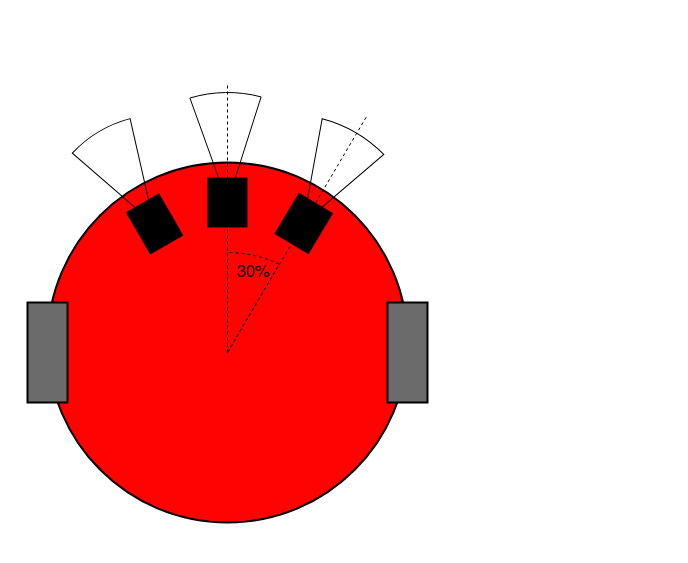
\includegraphics[width=0.5\textwidth]{UltraSoundSensorDiagram}
	\caption{Ultrasound Sensor Layout}\label{UltraSoundSensorDiagram}

\end{figure}

\subsection{Implementation}\label{elec/range/impl}
Sensor layout (3 deg cones)
circuit layout
schematic

The hardware required for the ultrasonic sensors is relatively straightforward. 
They are each connected to a \SI{5}{\volt} supply and ground, and the other two pins are 
connected to standard GPIO pins on the RPi. The echo pin has to be connected through 
a voltage divider as the RPi is only rated at \SI{3.3}{\volt} compared to the sensor's \SI{5}{\volt}. The 
trig pin can be connected directly to the RPi, however, as \SI{3.3}{\volt} was found to be above 
the threshold voltage.

The distances are measured by an \textit{USScan} class. This has a \textit{get
\_scan()} function which iterates through each ultrasonic sensor and takes a reading, 
as shown below in Code Listing \ref{lst:get_scan}

\begin{lstlisting}[caption={get\_scanFunction in USScan},label={lst:get_scan} , language=python]
def get_scan():
    """Get scan of ranges from all ultrasonic sensors.
    :return: (USScan) Scan of ranges
    :except: (UltrasonicTimeout) If module timed out waiting for GPIO input change
    """
    start = time.time()
    rl = get_range(LEFT)
    time_remaining = start + scan_increment - time.time()
    if time_remaining > 0:
        time.sleep(time_remaining)
    rc = get_range(CENTRE)
    time_remaining = start + 2 * scan_increment - time.time()
    if time_remaining > 0:
        time.sleep(time_remaining)
    rr = get_range(RIGHT)
    return USScan([rl, rc, rr])
\end{lstlisting}

This method allows the various readings to be taken without interfering with each other, as the second ultrasonic pulse isn't omitted until the first is received.

As \ref{lst:get_scan} shows,\textit{get\_range()} is used by
\textit{get\_scan()} to find the distance measured by each sensor.
This simply triggers the sensor and times how long until the echo
pin turns high. The range is then calculated by the equation
$ 2d = tv_s$ where $v_s$ is the speed of sound. It is then converted
to mm.

\subsection{Testing}\label{elec/range/test}
The sensors were initially tested using a signal generator and an
oscilloscope. An object was then placed in front of the sensors
and moved away. The expected output of this test was a linear increase
in the width of the pulse width on the echo pin as the distance
increased. This experiment allowed us to quickly identify 2
malfunctioning sensors. The pulse width could then be used to to
calculate the measured distance and this compared to the distance
found with a measuring tape. This found approximately correct answers,
however the precision with which we could measure the pulse width was
not great enough for effective testing.

The wave forms produced are shown in Figure~\ref{UltrasoundWaveform}.
This shows the shorted echo pulse following the fall of the wider
square wave on the trig pin, produced by the signal generator.

\begin{figure}[!ht]
	\centering
	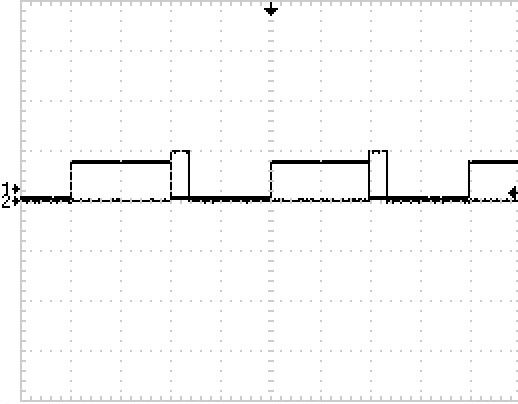
\includegraphics[width=0.5\textwidth]{graphs/UltrasonicResponseGraph.jpg}
	\caption{Ultrasound Response Waveform}\label{UltrasoundWaveform}

\end{figure}

A circuit was then created to read the values using an Arduino
microcontroller to allow the distance readings to be found quickly
and the accuracy of the sensors measured. The readings from this were
found to be approximately accurate (to at least within a half a cm,
as measured with a tape measure), although rigorous testing was not
performed as the accuracy would be dependant on the temperature due
to changes in air pressure, and we had no way of accurately controlling
this.

The testing was then repeated using the RPi set-up as to test the
software, with similar results obtained.

\section{Encoders}\label{elec/encoder}
Wheel encoders are required to measure the speed of each wheel
independently. This gives the system far more control over its path
as well as allowing it to perform dead reckoning through wheel odometry.

\subsection{Design}\label{elec/encoder/design}
The motors selected had both incremental and absolute custom designed
encoder, but as only the wheel speed is needed and not the position,
the incremental rotary encoders were used. These were hall effect
encoders, which measure the changing magnetic field of magnets which
are attached to the motor shaft. It has two 6 pole magnets magnets
which create 12 counts per revolution of the motor shaft, which, after
scaling for the gear ratio of 120:1, results in 1440 counts per
revolution of the robot wheel.

The encoders are quadrature encoders, which represent the speed and
direction of the wheels with two square waves where the frequency
represents the speed and which of the two waves is leading shows the
direction.

\subsection{Implementation}\label{elec/encoder/impl}

The encoder data was read into the RPi by an encoder class written in
Python. This worked by connecting call back methods to both the A and B
channel pins. How this is initialised is shown in Code Listing
\ref{lst:enc_event_detect}

\todo{format listings}

\begin{lstlisting}[caption={encoder callback set-up},label={lst:enc_event_detect} , language=python]
GPIO.add_event_detect(self.pin$_$a, GPIO.BOTH, callback=self._callback_a)
\end{lstlisting}

This then either increments or decrements a count depending on the
direction, as shown in Code Listing \ref{lst:enc_callback}. Note that
\textit{\_callback\_b()} is identical but with \textit{self.\_inc()} and
\textit{self.\_dec()} switched.

\begin{lstlisting}[caption={Encoder Callback Function},label={lst:enc_callback} , language=python]
def _callback_a(self, _):
        a, b = GPIO.input(self.pin_a), GPIO.input(self.pin_b)
        if a == b:
            self._inc()
        else:
            self._dec()
\end{lstlisting}


\subsection{Testing}\label{elec/encoder/test}
The encoders were first tested to ensure that they functioned correctly
using a test circuit and connecting the encoder outputs to an
oscilloscope. All the encoders were shown to function correctly
outputting square waves in both channels and with channel A leading B
when the motor was moving forwards and B leading A when going forwards.
\todo{check order}

An example of the encoder output found is shown in Figure
\ref{EncoderGraph} below. This shows the two square waves produced by the
two encoder outputs a quarter wavelength out of phase.

\begin{figure}[!ht]
	\centering
	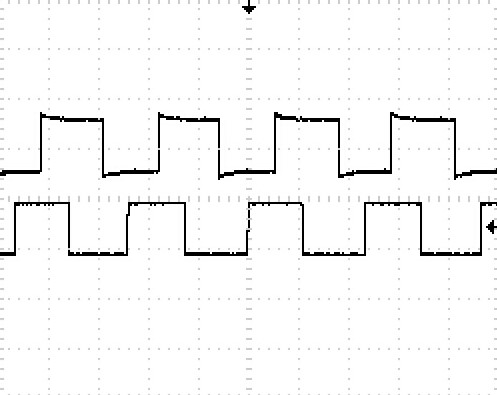
\includegraphics[width=0.5\textwidth]{graphs/EncoderGraph.jpg}
	\caption{Encoder Output Test Waveforms}\label{EncoderGraph}

\end{figure}

This experiment allowed us to quickly confirm the correct functionality
of all 6 encoders, however did not allow us to test the accuracy. After
this, the motors were run at a low speed for several rotations while the
system counted pulses. This was not an accurate test of the encoders, as
the wheel could not be stopped at an exact integer multiple of rotations,
however did verify that the system was approximately outputting 1440
counts per rotation.

\section{IMU}\label{elec/imu}
The IMU consists of a three axis accelerometer and a three axis gyroscope
which can be used to measure both the linear acceleration and rotational
velocity of the robot. This can be integrated and double integrated to
track the robots position over time again performing dead reckoning. The
system can then perform sensor fusion on this data and the encoder
readings to get far more accurate results than possible with either system
independently.

\subsection{Design}\label{elec/imu/design}
The IMU selected was the MPU-6050. It was the most accurate sensor of a
similar budget with regards to noise, cross axis sensitivity and non
linearity. Offset tolerance was also considered but this was less of a
consideration as this can be compensated for as long as the offset is not
so extreame as to limit the range. It was configured to operate in its
smallest range of values ($\pm\ang{250}s^{-1}$ and $\pm2g$\cite{}\todo{citation}).

The IMU was to be placed as close to the centre of the axis of the robot
as possible, as when it is far from the centre of rotation the centripetal
forces acting on it can interfere and be measured as linear motion away
from the centre.

\subsection{Implementation}\label{elec/imu/impl}
The IMU selected uses the I$^2$C protocol for data transmission, which
integrates well with the RPi as it has dedicated I$^2$C GPIO pins and
existing libraries to facilitate communication.

It should be noted that, while this was the only I$^2$C device currently
used, other devices with conflicting addresses can be handled as The IMU
allows the address to be changed through a data pin from 0x68 to 0x69.
This would most likely be used if the framework developed was being used
on another, more complicated system requiring several IMUs. This pin was
not connected to the RPi in this design as it was not yet required.
\todo{code description}

An \verb|i2c_object| class that used the smbus package was created to
simplify the communication over the I\textsuperscript{2}C buses. These
were initialised with an I\textsuperscript{2}C bus and an address, and
contained various methods for reading and writing to the I
\textsuperscript{2}C device.

\todo{what code is interesting}

An \verb|IMU| class was then created to read the data from the IMU which
and an \verb|i2c_object| instance. Code Listing \ref{lst:imu_init} shows
the constructor for the IMU class. Note that the \verb|write_byte()| call
is essential to enable the IMU transmissions.

\begin{lstlisting}[caption={IMU Initialisation Function},label={lst:imu_init} , language=python]
def __init__(self, address, rate, channel=1):
    self.address = address
    self.IMU_i2c = i2c.i2c_object(self.address, channel=channel)
    self.rate = rate
    self.IMU_i2c.write_byte(0x6B, 0x00) # turns imu on
    self.speed_vect = (0.0, 0.0, 0.0)
\end{lstlisting}

As the IMU returns arbitrary values between -32768 and 32767
\todo{source}, a constant was required to convert the results to
meaningful values. The calculations for these is shown in Code
Listing~\ref{lst:imu_units}.

\begin{lstlisting}[caption={Calculation for IMU Value to SI unit Conversion Constants},label={lst:imu_units} , language=python]
GYRO_RANGE = 250  # deg/sec
GYRO_DIVISIONS = 32768  # 2 ^15
GYRO_UNITS = (GYRO_RANGE * math.pi * 2.0) / (GYRO_DIVISIONS * 360)  # rad/sec

ACC_RANGE = 2 * 9.81  # m/s^2
ACC_DIVISIONS = 32768  # 2 ^15
ACC_UNITS = ACC_RANGE / ACC_DIVISIONS  # m/s^2
\end{lstlisting}

The acceleration values can then be multiplied by the \verb|ACC_UNITS|
constant and the result is the acceleration in $ms^{-2}$, and \verb|GYRO_UNITS|
can be used similarly to find the rotation in $rads^{-1}$, as is
shown in Code Listing \ref{lst:read_funcs}.


\begin{lstlisting}[caption={Reading and Converting Raw IMU Values},label={lst:read_funcs} , language=python]
    def _read_gyro(self):
        x_rot_v = self.IMU_i2c.read_signed_word(0x43) * GYRO_UNITS
		...
        return (x_rot_v, y_rot_v, z_rot_v)

    def _read_accel(self):
        x_a = self.IMU_i2c.read_signed_word(0x3b) * ACC_UNITS
		...
        return (x_a, y_a, z_a)
\end{lstlisting}

The final step in reading the IMU results is to integrate the acceleration
data as to get the linear velocities. This makes use of the \textit{speed
\_vect} variable declared in the IMU constructor shown in Code Listing
\ref{lst:imu_init}. \textit{speed\_vect} is incremented by the
acceleration multiplied by the IMU rate, as shown in
\ref{lst:imu_integration}.

\begin{lstlisting}[caption={Integrating Linear Acceleration},label={lst:imu_integration} , language=python]

def get_speeds(self):
		...
        accel_vect = self._read_accel()
        speed_vect = tuple([(1.0/self.rate) * accel_vect[i] + speed_vect[i] for i in range(len(accel_vect))])
        return speed_vect, gyro_speeds
\end{lstlisting}


\subsection{Testing}\label{elec/imu/test}
Initial work was performed with the IMU and an Arduino microcontroller before the RPis were acquired. The IMU was connected up and various movements were recorded. Python code was then written to interpret and visualise the data as a moving frame.

\section{PCB}\label{elec/pcb}
As precise and consistent placement of components was required to ensure homogeneity of the robots, it was decided to develop a PCB for the connection and mounting of the parts (as opposed to using strip board). The following describes the rationale and design decision taken when carrying out the 3-iteration design process for designing the PCB. The final PCB design can be found in the git repository (see Section~\ref{appendix/a}).\todo{ensure this is where the git link is}

\subsection{Design}\label{elec/pcb/design}
The PCB required to contain the following components:
\begin{itemize}
  \item Raspberry Pi ribbon cable connector
  \item Three ultrasonic sensors
  \item IMU
  \item Left and right encoder connectors
  \item Motor drive connectors
  \item Power connectors
  \item LEDs for debugging
\end{itemize}

with the following physical design constraints:

\begin{itemize}
  \item Central ultrasonic sensor at the centre of the robot in the x axis
  \item the other ultrasonic sensors symmetrical about the y axis
  \item IMU chip in centre of axis
  \item Mounting holes for RPi and for mounting PCB to chassis
  \item Power connectors at fixed position relative to centre to ensure it connects to header on power distribution board
  \item Motor drive connectors also at fixed position relative to centre
\end{itemize}

\begin{table}[!ht]\centering
\caption{Pin assignments for iterations of the PCB design
\label{table:pin_assignments}}
    \begin{tabular}{ccccc}
        \toprule
        \thead{Pin} & \thead{Description} & \thead{PCB v1\\(Blinky)} & \thead{PCB v2\\(Inky)} & \thead{PCB v3\\(Clyde)}\\
        \midrule
        GND & Ground                 & 9  & 9  & 9  \\
        VCC & \SI{5}{\volt} supply   & 2  & 2  & 2  \\
        MLD & Left motor DIR         & 11 & 11 & 11 \\
        MLP & Left motor PWM         & 32 & 32 & 32 \\
        MRD & Right motor DIR        & 15 & 21 & 19 \\
        MRP & Right motor PWM        & 33 & 33 & 33 \\
        MS  & Motor SLP              & 13 & 13 & 13 \\
        ULT & Left ultrasonic TRIG   & 35 & 35 & 35 \\
        ULE & Left ultrasonic ECHO   & 37 & 37 & 37 \\
        UCT & Centre ultrasonic TRIG & 16 & 16 & 16 \\
        UCE & Centre ultrasonic ECHO & 12 & 12 & 12 \\
        URT & Right ultrasonic TRIG  & 22 & 22 & 22 \\
        URE & Right ultrasonic ECHO  & 18 & 18 & 18 \\
        ELA & Left encoder A         & 23 & 23 & 21 \\
        ELB & Left encoder B         & 19 & 19 & 23 \\
        ERA & Right encoder A        & 24 & 24 & 24 \\
        ERB & Right encoder B        & 26 & 26 & 26 \\
        LG  & Green LED              & 31 & 31 & 31 \\
        LR  & Red LED                & 29 & 39 & 29 \\
        SDA & \isc{} SDA (IMU)       & 3  & 3  & 3  \\
        SCL & \isc{} SCL (IMU)       & 5  & 5  & 5  \\
        \bottomrule
    \end{tabular}
\end{table}

\todo{Rationale for pin choices and why they were changed}

With these constraints the following PCB design shown in figure \ref{PCB_Design}.

\begin{figure}[!ht]
	\centering
	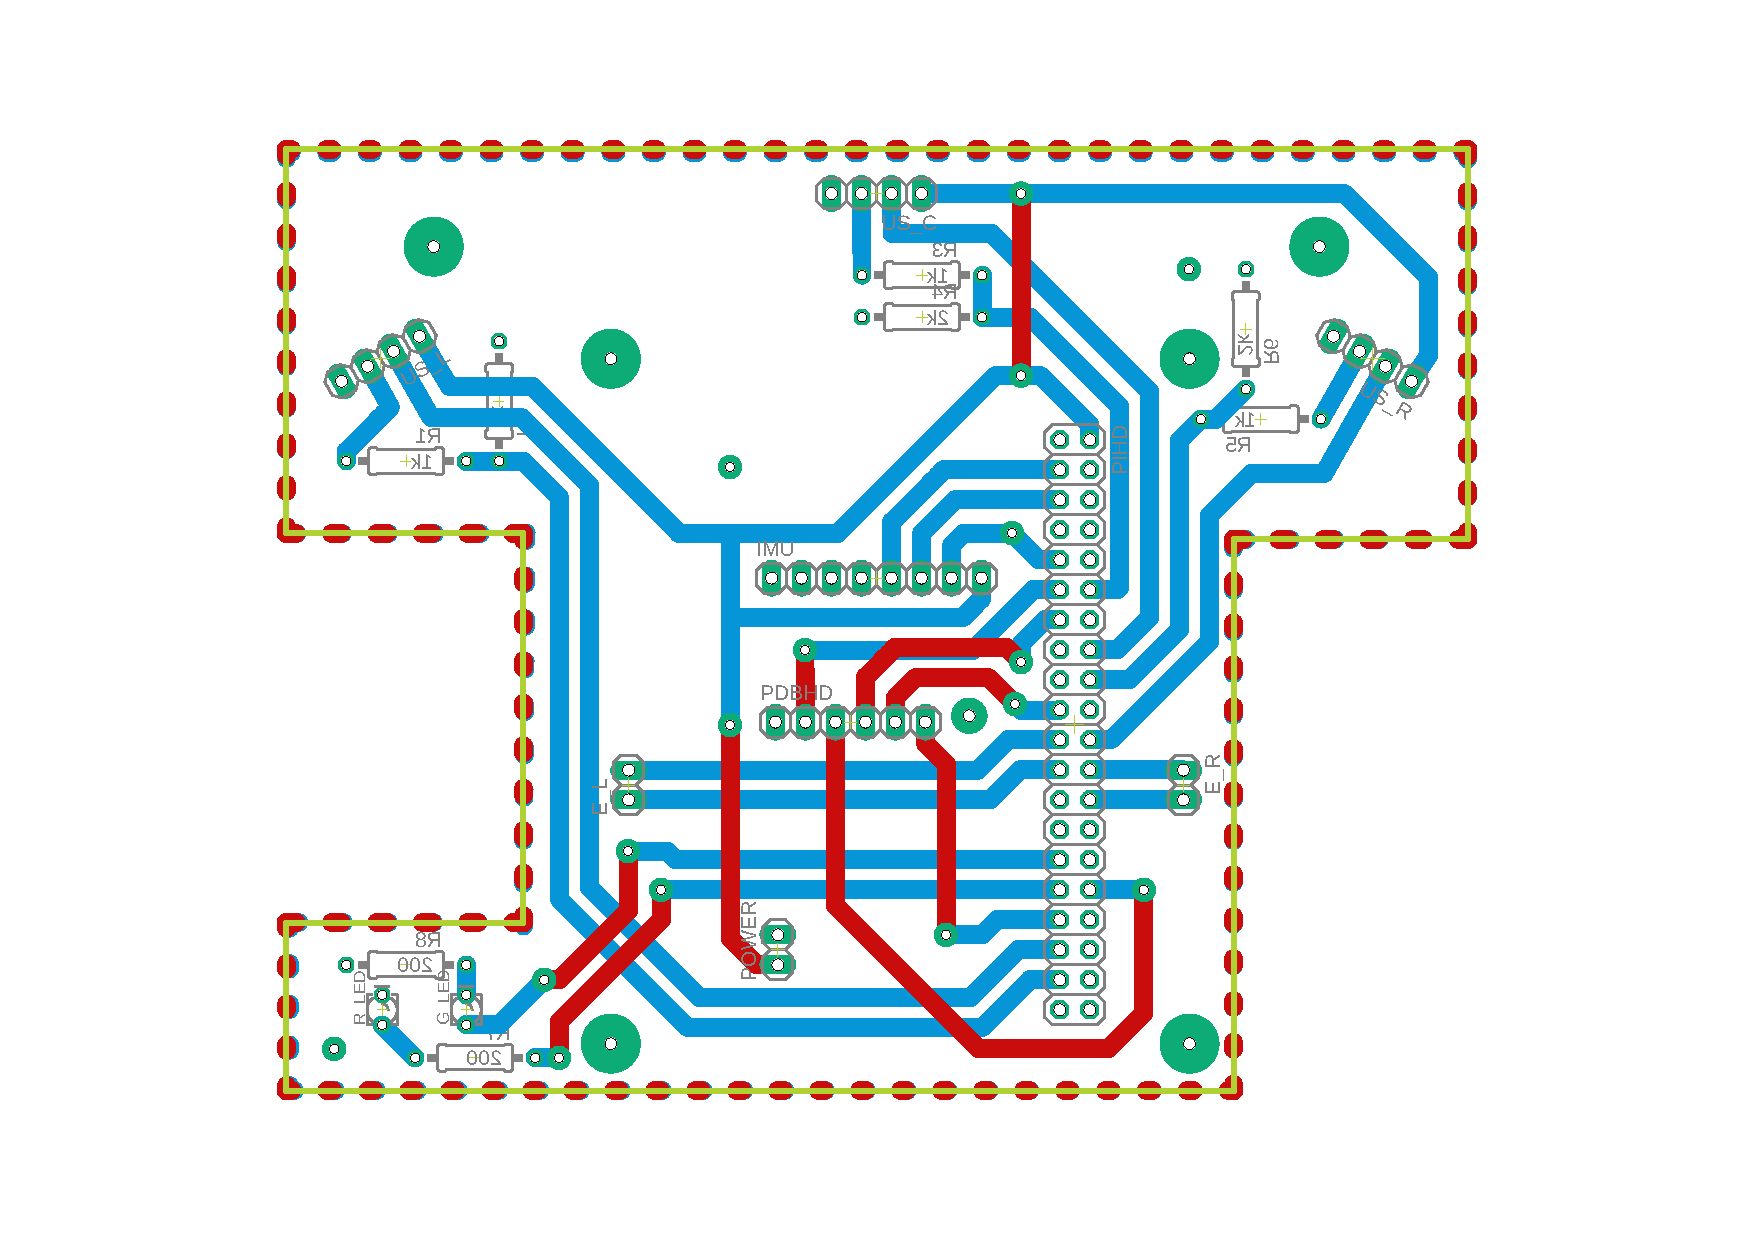
\includegraphics[width=1\textwidth]{main_pcb.pdf}
	\caption{Final PCB Design}\label{PCB_Design}

\end{figure}
Note that the peculiar shape is to allow room for the motors and encoders.

\subsection{Testing}\label{elec/pcb/test}
After the components were soldered into place on the PCB, manual
continuity tests were performed with a multimeter to ensure that adjacent
pins had not been connected in the soldering process.

The PCB was then mounted and each module test was rerun to ensure that the
connections were all correct. This process exposed a flaw as one of the
ultrasonic sensors seemed to no longer work. After some investigation it
was noticed that the screws being used had slightly larger heads than the
screws used for mounting the test strip board and was connecting two
tracks. A rubber washer was used as temporary fix and then this was
corrected in the final PCB design.

    % !TEX root = ../report.tex

\chapter{Software}\label{software}
The software architecture was centred on the event driven implicit implication 
design pattern~\cite{garlan1993introduction}. This architecture design pattern is 
also known as the ``Hollywood'' design pattern due to its definition of ``Don't 
call us, we'll call you''. With regards to software architecture this means 
modules are signalled to start by other modules and this is propagated through 
the system with ``events'' triggering other ``events'' within the system. 

To implement this architecture, each part of the system can be defined as its own 
module with a function which triggers its invocation and a function which can 
broadcast events if required. A methodology for implementation of this system is 
the publish/subscribe model. Each modules' invoking function is a publisher and 
modules which would be triggered by this function are known as subscribers. Using 
this method in the context of this project, means the software has strong support 
for reuse --- as new sensors or libraries can be plugged in and subscribe to the 
appropriate events --- and loose coupling throughout the system means that 
maintenance of each module can take place independently. 

In robotic systems, this architecture is highly beneficial as each of the sensor 
and actuator systems can run independently publishing their data for feedback, 
using event driven implicit invocation through data driven programming. This 
reduces the risk of system crashes as module crashes are isolated, improving 
robustness.   

\todo{Bit here about deploy.sh or a new section}

\section{ROS}\label{soft/ROS}
In order to implement this architecture, and following extensive research(see 
Section~\ref{litreview/ROS}, the Robot Operating System (ROS) library was 
selected as a framework. The ROS library makes it simple to design and implement 
individual modules within a system and uses a central control node named 
``roscore'' to manage publish and subscribe ``topics'' between modules. 

\subsection{Design}\label{soft/ROS/design}
Following the decision to use ROS to implement our chosen architecture, a modular 
approach was adopted for the design of each of the components within the system~
\ref{elec}. Hence, a system block diagram was developed to visualise data flow 
within the system. \todo{put in block diagram} The block diagram in Figure~
\ref{BlockDiagram} demonstrates the modularisation of the system and also the 
expectation that the AI module at the top of the system will be completely 
independent from the other components of the system. By making the control module 
an API, AI algorithms can be interchanged easily for testing. The modular 
approach also means sensor and actuator modules can be plugged in and out as 
desired and could easily be changed if needed at any point in the project. 

Each module can be programmed in a different language before being converted to a 
ROS node, which publishes and subscribes, using the appropriate methods for that 
language. Although the majority of the system will be programmed in Python, 
allowing different programming languages means that timing or processing 
sensitive operations can be programmed in C or C++ as required. Once converted to 
a ROS node, each module can then be started individually using a ROS launch file. 
Launch files are used by ROS to create and start a number of nodes within a 
system with any number of parameters. Again, due to the modular approach and use 
of ROS, launch files allow various configurations of modules to be tested easily.  

In order for ROS launch files to function, the directory structure within the 
``catkin''~\cite{catkin} workspace must be configured correctly. ``Catkin is the 
CMake based build system that is used to build packages in ROS''~\cite{gitcatkin} 
and requires a strict directory structure in order to build each of the 
individual modules within the project. Packages within ROS allow code to be 
maintained and compartmentalised, and by using packages throughout existing 
packages can be added easily. 

Considerations of appropriate packages were made and a final design UML diagram 
created\todo{UML~\ref{UMLDiagram}}. This demonstrates a full system 
implementation and the expected interactions between each of the modules within 
the program. 
\subsection{Implementation}\label{soft/ROS/impl}
Each of the individual modules discussed in Section~\ref{elec} were transformed 
into ROS nodes. These modules are implemented within Python scripts which can be 
run as ROS nodes. The following listing shows an example of how this was done 
with the .... node \todo{ listing here of example}. This listing shows the Python 
version of a ROS node, which is the case for the majority of the nodes. Although 
a variety of languages was permissible, in practice the majority of the code base 
is Python. The $spin()$ method is the ``main loop'' for each of the modules and 
carries out tasks while the node is running. Each of the nodes which publish 
information to the system also use the $rospy.Publisher$ class to create objects 
which can then publish messages of a pre-determined type to the system. 
Similarly, $rospy.Subscriber$ is used by nodes wishing to listen for messages on 
a specific topic. 

To further modularise the code for each node, object oriented Python was used and 
each node defined as its own class. This meant that each method within the class 
was defined for that class and function names could be repeated throughout the 
codebase where this made sense, such as with the $spin()$ method. Each node also 
has an $init()$ method which is called on instantiation of the class which it 
is contained within. This \todo{add init listing} example code shows the setup 
for the Motor node. A number of parameters are set or drawn in from the launch 
file from which the node was created and the node set as a subscriber to the 
$motor cmd$ topic which gives instructions to the Motor node. By using a number of parameters the code maintains its flexibility as these can be tuned in different launch files to different values. Topic values can also be changed on the fly using thje command line from within a catkin workspace, allowing real time tuning of parameters to take place. 
  \todo{David needs to write this i think}


\subsection{Testing}\label{soft/ROS/test}
In addition to each of the nodes being tested independently in a similar manner to how each of them were tested in isolation throughout the~\ref{elec} Section, the nodes were tested in a number of different configurations.  
\todo{David maybe needs to write this}

Each of the topics can be tracked from the main graph of nodes in the ROS runtime using the command $rqt graph$. This produces the following output, \todo{put rqt grpah of nodes and topics in here and dicuss}. 


\section{Communication}\label{soft/comms}

\subsection{Design}\label{soft/comms/design}

\subsection{Implementation}\label{soft/comms/impl}

\subsection{Testing}\label{soft/comms/test}




\section{SLAM \& Sensor Fusion}\label{soft/SLAM}

\subsection{Design}\label{soft/SLAM/design}

\subsection{Implementation}\label{soft/SLAM/impl}

\subsection{Testing}\label{soft/SLAM/test}



\section{Computer Vision}\label{soft/cv}
Computer vision is a very cheap and effective way of gaining a high level understanding of the environment. It was used to allow the agents to identify other robots and objectives in in the system. Detecting the other robots was an essential component to allow communication between robots, prevent agents mistakenly mapping other agents,and to recognise when ultrasonic interference would occur. 

\subsection{Design}\label{soft/cv/design}
The first detection system considered was a CNN, as discussed in Section \ref{litreview/cv/objDet/CNN}. This is a very effective system which has the advantage of 
being able to classify instances of objects that it has not 
seen before. This would be essential if the target objects of 
the robot was not consistent, for instance if it had to find 
people in the search space. This was, however, not essential 
in the scope of this project. The major downside to this 
system would be the time to implement. To construct a CNN for 
this application would require the collection of a large data 
set of images of the robots and goals, as well as the time 
consuming process of tuning the CNN. 

Feature Based Object detection was also considered. As described in Section \ref{litreview/cv/objDet/fb}, this only requires a picture to be taken of the object and therefore takes far less time to 
implement than the CNN solution. However, the accuracy and 
consistency are largely dependant on the number of features 
detected, and the algorithm's complexity grows relatively 
quickly. The basic brute force algorithm involves comparing 
every key point in the object image to every key point in the 
frame image, which results in an O($n^2$) complexity (although 
this can be streamlined, for instance if it becomes impossible 
for the distance to be low enough for a pair to be the best 
match part way through the distance calculation, it does not 
need to be finished). The calculations for deciding the best 
outline of the object also become more complicated, as there 
will be a lower true positive to false positive ratio as the 
best matches (which are found first) are more likely to be 
true positives. It was decided that this would be too  
computationally intensive considering the strict constraint of 
using a Raspberry Pi. 

The method used was by far the simplest considered. It identified the other robots and target by their colour. This was only possible as each robot used had a distinct coloured chassis, which lacks scalability, but was considered an acceptable simplification as this was not the focus of the project. 

This works by first converting the images from RGB to Hue-Saturation-Value (HSV) colour space, simplifying the colour detection as the hue of the pixel is determined by a single value instead of the ratio of three values. A colour can then be identified by a range of H values and then a minimum S and V values, which is far more intuitive than checking if it falls into a range of ratios between R, G and B values. 

\subsection{Implementation}\label{soft/cv/impl}
The \textit{vision\_node} works using a ROS spin setup, with a \textit{spin()} function being called at a set frequency until ROS closes. 

A \textit{RobotDetector} object is declared which has the range of HSV values for each robot and the goal, and has a video capture object. It contains a \textit{search()} function which takes a frame as a parameter and returns various details about each robot's presence in the frame. \textit{search()} first calls \textit{get\_colour\_mask()} for each range of colour values. This converts the image to HSV, then makes a frame, \textit{mask}, which is white where the pixel in range and and black for out of range. This is shown in Code Listing \ref{lst:get_colour_mask}. This also shows the handling of cases where the range of colours crosses the zero point (as zero is adjacent to 255 in the hue value).

\begin{lstlisting}[caption={get\_colour\_mask in RobotDetector},label={lst:get_colour_mask} , language=python]

def get_colour_mask(self, frame, lower_hsv_bound, higher_hsv_bound):
        hsv_frame = cv2.cvtColor(frame, cv2.COLOR_BGR2HSV)

        if (lower_hsv_bound[0] > higher_hsv_bound[0]):
            mask1 = cv2.inRange(hsv_frame, np.array([0, lower_hsv_bound[1], lower_hsv_bound[2]]),
                                np.array(higher_hsv_bound))
            mask2 = cv2.inRange(hsv_frame, np.array(lower_hsv_bound),
                                np.array([179, higher_hsv_bound[1], higher_hsv_bound[2]]))
            mask = mask1 | mask2
        else:
            lower = np.array(lower_hsv_bound)
            upper = np.array(higher_hsv_bound)
            mask = cv2.inRange(hsv_frame, lower, upper)

\end{lstlisting}

The function then uses erosion and dilation functions provided by opencv to reduce noise in the mask. 

The contours in the mask are then iterated through to find the biggest, which is assumed to be the object and the centre point and outline of the contour is found. If no contours are bigger than a fixed size (measured in pixels) the object is assumed to not be in the image frame, and the corresponding \textit{obj\_found} variable is set to false. This process is shown in Code Listing \cite{lst:cv_search_loop}.

\begin{lstlisting}[caption={Contour Iteration in search()},label={lst:cv_search_loop} , language=python]
...
for c in contours:
    if cv2.contourArea(c) > max((300, maxsize)):  
        maxsize = cv2.contourArea(c)
        cx, cy = self.get_centre_point(c)
        outline = self.get_outline(c)
        obj_found = True
...
\end{lstlisting}

These parameters are then returned to the \textit{\_tick()} function which was called by \textit{spin()}. This then renders debug info to the frame if it's performing a test, or publishes the detected robot info via a ROS message consisting of a comma separated list of objects detected in the last frame. 

\subsection{Testing}\label{soft/cv/test}
Initial testing of the \textit{vision\_node} was performed on a PC with a USB webcam. The testing was performed by using the position information to render labelled rectangles to a real time stream highlighting the position of the objects. The code for this is shown in Code Listing \ref{lst:draw_rectangles}. 

\begin{lstlisting}[caption={asd},label={lst:draw_rectangles} , language=python]
for i, name in enumerate(names):
    if found[i]:
        #cv2.drawContours(frame, [outline], -1, (0, 255, 0), 2)
        #cv2.circle(frame, (cx, cy), 7, (255, 255, 255), -1)
        x, y, w, h = cv2.boundingRect(outlines[i])
        cv2.rectangle(frame, (x, y), (x + w, y + h), highlight_colours[i], 2)
        cv2.putText(frame, name, (x - 20, y - 20),
                            cv2.FONT_HERSHEY_SIMPLEX, 0.5, highlight_colours[i], 2)
\end{lstlisting}

An example of this running is shown in Figure \ref{fig:cv_screenshot}

\begin{figure}[!ht]
	\centering
	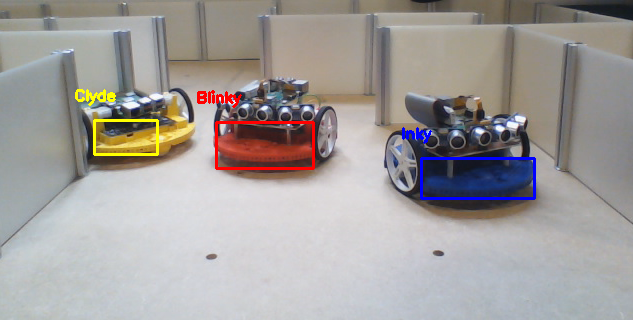
\includegraphics[width=1\textwidth]{ComputerVisionScreenshot.png}
	\caption{Computer Vision PC Test}\label{fig:cv_screenshot}

\end{figure}

The system was then tested on the RPi by monitoring the ROS topic \textit{robots\_detected} to test both the integration with the RPi and with ROS. Various detectable objects were moved in and out of the frame and changes in the output were observed. This initially failed as the RPi camera was connected using a CSI port, not a USB port, which OpenCV's VideoCapture function does not support. When running on the RPi, this was replaced with imutil's VideoStream package. After this the test performed as expected, consistently identifying which objects were in frame.  

Functionality was then added to record the feed as to see how the computer vision responded as the robot was traversing the maze, however there were issues with frame rate as it was too computationally intensive for the RPi to perform the recording as well as all the other computation. 

\section{AI \& Control Modules}\label{soft/ai}

\subsection{Design}\label{soft/ai/design}

\subsection{Implementation}\label{soft/ai/impl}

\subsection{Testing}\label{soft/ai/test}
    % !TEX root = ../report.tex

\chapter{System Testing}\label{systest}
System testing took place following integration testing and
the full construction of the robot. The aim of system testing is to ensure that
each of the component parts work as expected when integrated together, and to
test and evaluate the system as a whole. A modular
maze testing environment was used throughout integration and
system testing to allow as many different maze configurations
as possible to be tested. Throughout integration the modular maze was used as a
``SLAM playground'', where various sized boxes or simple two area configurations
were used to test the robot's capabilities in these environments and assess the
SLAM maps built when using these configurations.
\section{Modular Maze}\label{test/maze}
The modular maze environment was designed with the aim of being able to system
test on as many maze configurations as possible. By creating a modular
environment, the maze was also reusable in future iterations of the project, or
similar projects which required a secure area to test small autonomous vehicles.
\subsection{Design}\label{test/maze/design}
With these broad specifications in mind, a list of requirements for the maze
environment was created (see Table~\ref{maze_reqs}).

\begin{table}[!ht]\centering
\caption{Modular Maze Requirements
\label{maze_reqs}}
    \begin{tabular}{ccc}
        \toprule
        \thead{Requirement} & \thead{Priority}\\
        \midrule
        Be easily modifiable & High\\
        Have enough cells to allow varied mazes & High\\
        Have minimum cell width $>$ diameter of the robot & High\\
        Be accompanied by sufficient ``pegs'' and ``walls'' to build complex 		mazes & High\\
        Wall material be non-translucent and non-reflective & Medium\\
        Base material be non-reflective & Medium\\
        Maze be easily transportable & Medium\\
        Maze base be modular & Low\\
        \bottomrule
    \end{tabular}
\end{table}

These requirements were then used to create a number of approximate ideas which
were presented to the mechanical workshop. The maze base would be \SI{1280}{\mm}
$\times$ \SI{1690}{\mm} $\times$ \SI{18}{\mm}, giving 7 columns by 9 rows of
peg holes each \SI{12}{\mm} in diameter and \SI{210}{\mm} from centre to
centre. The holes drilled into the maze base would be \SI{15}{\mm} in depth
leaving a \SI{3}{\mm} section of the base board un-drilled within the hole for the peg to rest on. The ``pegs'' would then be
\SI{165}{\mm} in height, a protrusion of \SI{150}{\mm} from the top of the base board, with a cross slit cut from the top to
roughly \SI{75}{\mm} down the peg
(half the visible portion). These slits would be approximately \SI{3}{\mm} wide to allow the walls to be slotted in. In order for
this to be accomplished, the walls would be winged --- \SI{208}{\mm} in length at the top and \SI{196}{\mm} in length,
\SI{75}{\mm} from the top. This gives \SI{6}{\mm} spaces at either side to allow for the diameter of the peg and means the walls
can be slotted between two pegs with ease.

The materials required were researched in order to obtain the measurements
above, such as \SI{12}{\mm} being a standard size for wood dowel and \SI{3}{\mm}
and \SI{18}{\mm} respectively being depths of MDF which could be used for the
walls and base boards. These requirements, descriptions and accompanying
drawings were delivered to the mechanical workshop for construction to begin.

\subsection{Implementation}\label{test/maze/impl}
The mechanical workshop required a number of changes to the original design in
order for the maze to be created.

Foremost, the largest single item of solid wood which could be obtained from
suppliers was smaller than the requested measurements of \SI{1280 x 1690 x 18}
{\mm}. Two resolutions were proposed by the mechanical workshop: reduce
the width of each cell, or remove a column of holes from the maze. Following
team consultation, it was decided that reducing the size of each cell would
result in more flexibility in the end product, as 3 columns of two cell wide paths could still
be created. It is also worth noting that the reduced cell width of \SI{195}{\mm}
still met the requirement of the cell width being larger than the diameter of
the robot.

Secondly, the materials used for the walls and pegs would not be wood as this
would involve a number of man hours to create the slits in the dowel and
manually cut the walls to size. In order to streamline the process, it was
suggested by the mechanical workshop, that the walls be made of acrylic, allowing
them to be laser cut, and the pegs be 3D printed, allowing mass printing
once a design had been finalised. It was agreed amongst the group that this was a good idea and
in order for the pegs to be 3D printed they had to be made using CAD modelling
software. None of the group had particular experience using this software, hence
a steep learning curve was involved in carrying out this task.

A peg matching the original specifications was modelled, however upon delivery
to the mechanical workshop, the group were informed that this designed had
changed to allow the walls to be cut as rectangles only --- with no wings. A new
peg design was created which had slits at each \SI{90}{\degree} interval,
running the length of the peg. This allowed the wall to be dropped in without
the need for wings. This peg design was also modelled.

Upon returning to the mechanical workshop the group were once again informed
that the peg design had to be altered. The base board had been drilled through
and so the pegs now required a smaller peg on the bottom and a rim to ensure
that they did not fall through the base board. The agreed design was the same as
previously with the peg now having a diameter of \SI{15}{\mm} with the small peg
at the bottom having the original \SI{12}{\mm} diameter and \SI{15}{\mm} in
height. The design was agreed and the peg was modelled.

Midway through modelling the group were called by the mechanical workshop and
informed that the perspex which had been ordered was slightly wider than the
originally thought \SI{3}{\mm} and so the slits would have to be widened to
\SI{4}{\mm} to allow for this. The model was altered to account for this change and delivered to the mechanical workshop to be 3D printed.

Unfortunately, once printed it was discovered that the design resulted in a peg
that was too fragile and often broke at the base. The mechanical workshop
attempted to resolve this issue by increasing the density of the printing,
however this was unsuccessful. Eventually, the mechanical workshop concluded
that ordering a pre-slitted rod of aluminium and attaching metal pegs to the
base to allow them to fit into the base board would be the best solution. This
solution was successful and the maze with 53 pegs and 52 walls was
delivered in full shortly afterwards. An example configuration of the maze is shown in Figure~\ref{fig:maze_pic}.

\begin{figure}[!ht]
	\centering
	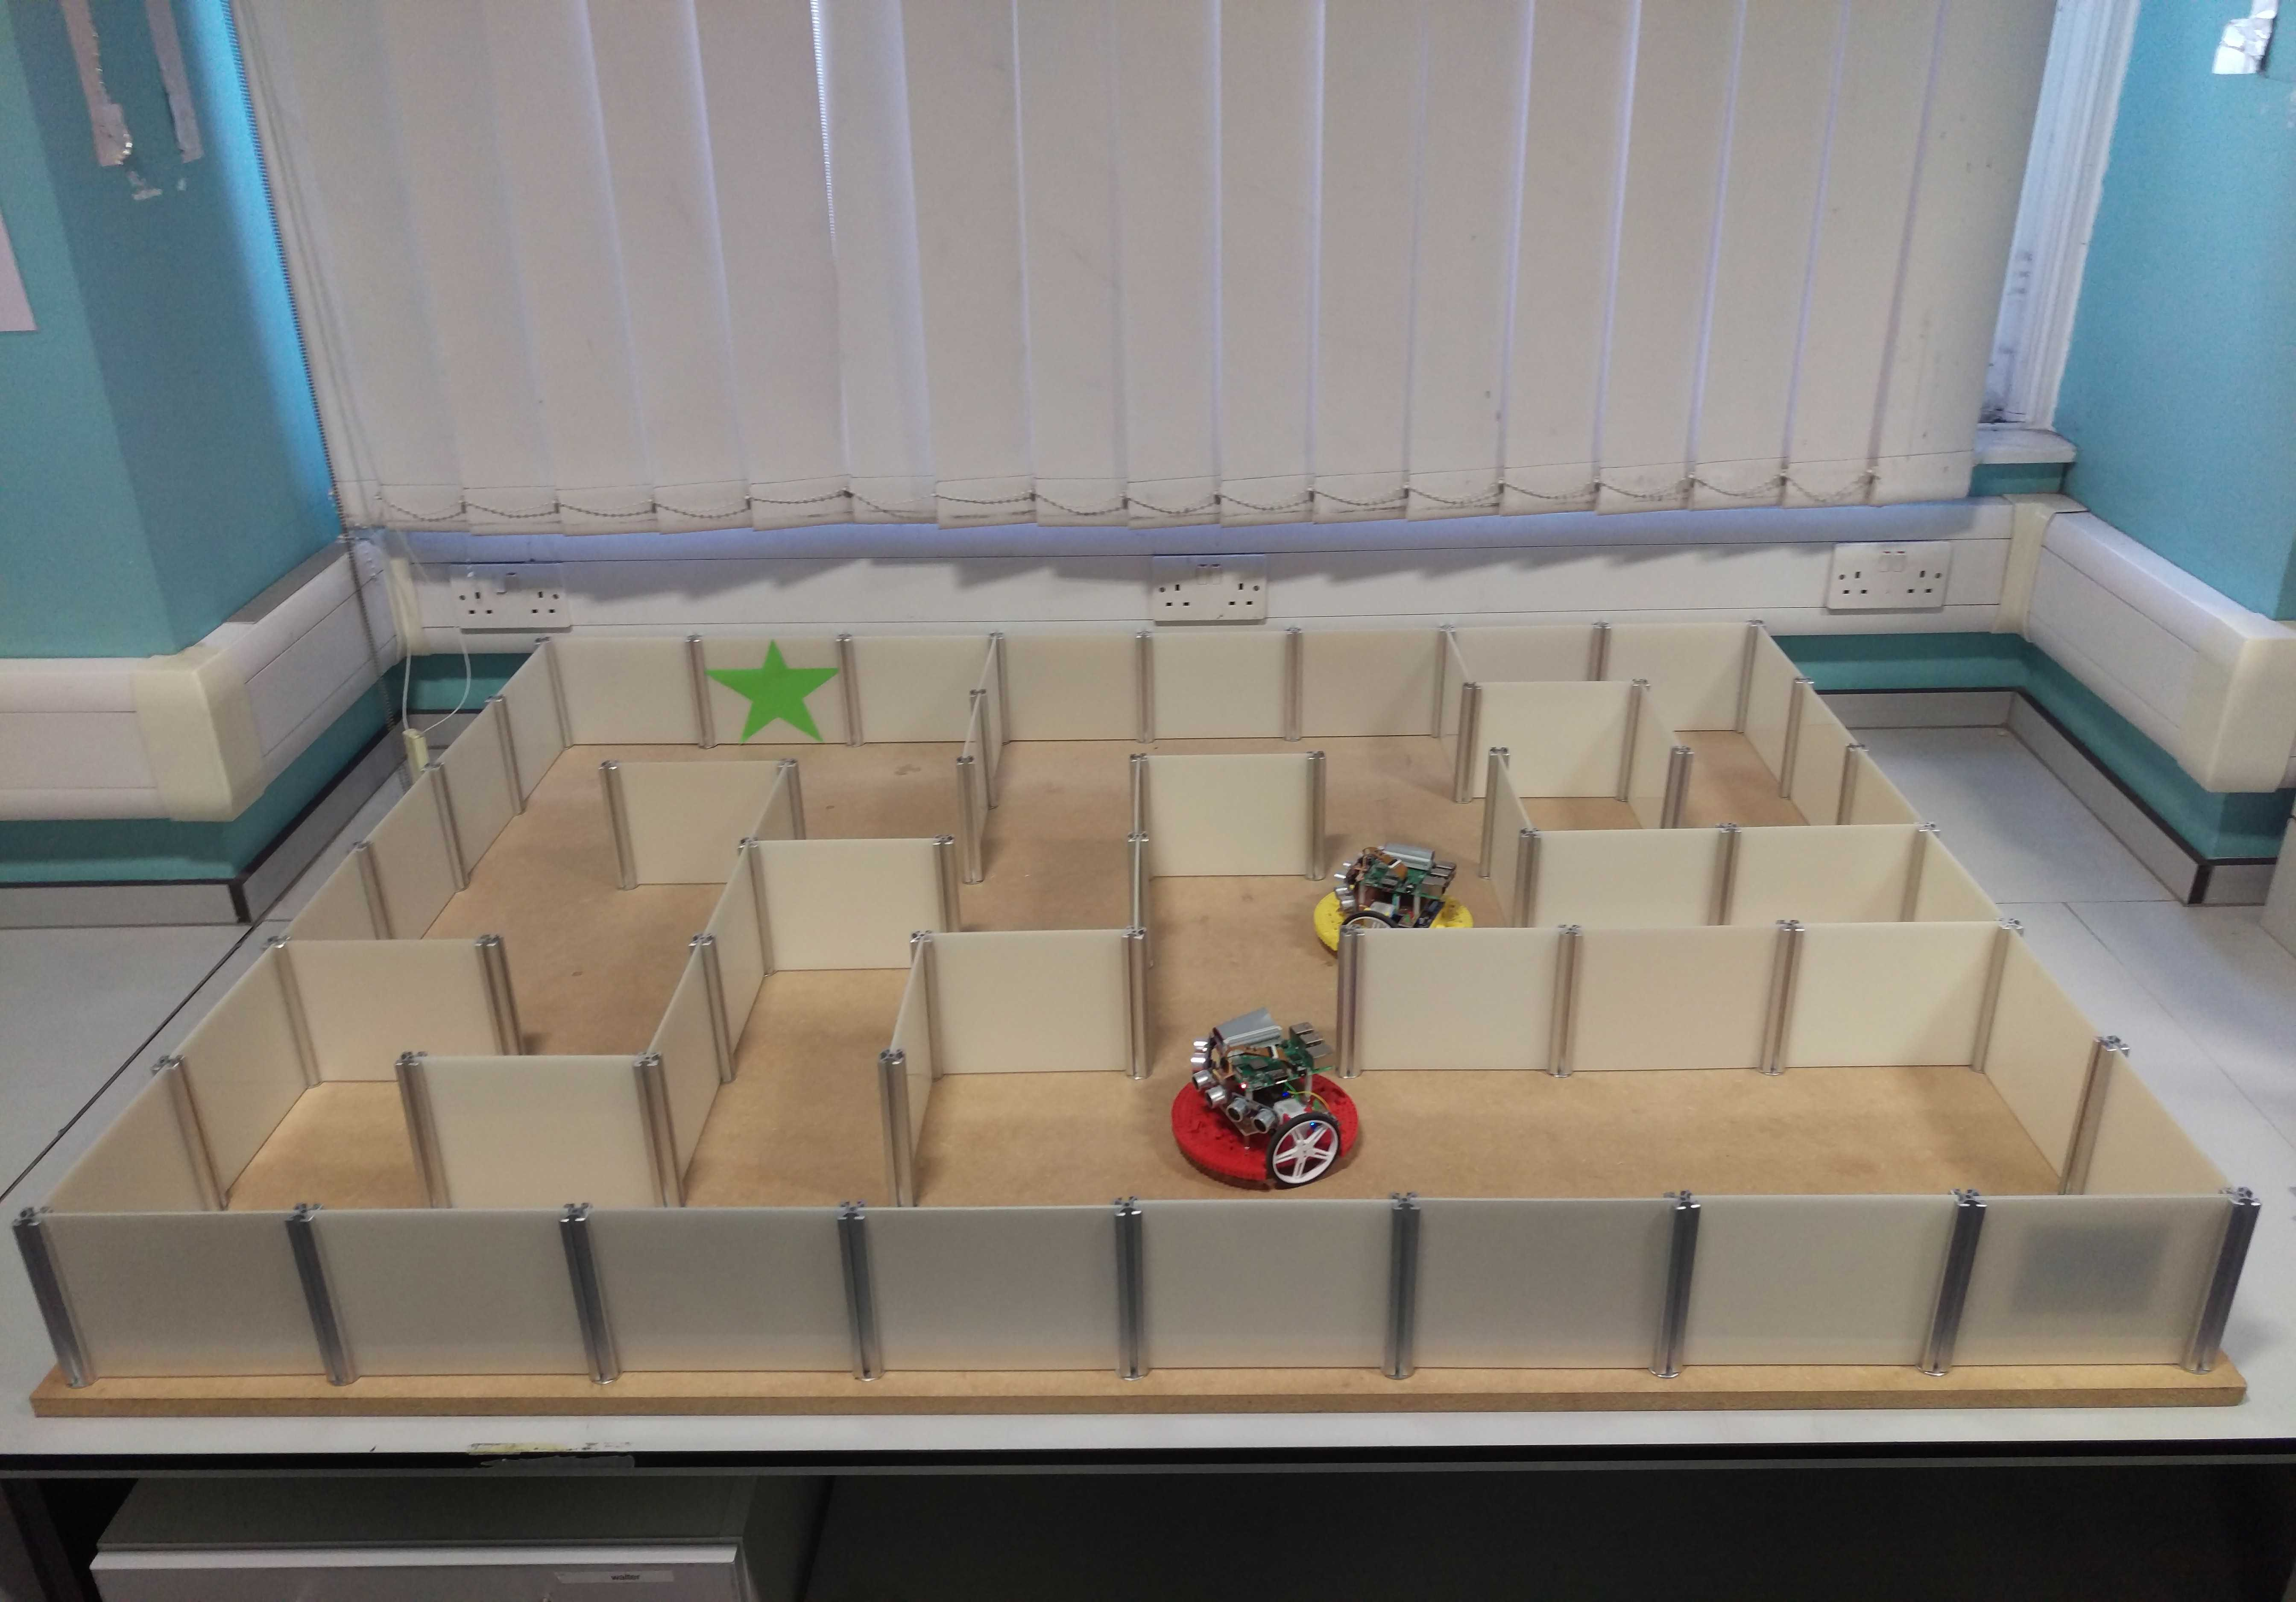
\includegraphics[width=0.8\textwidth]{diagrams/Maze4Real}
	\caption{An example maze configuration constructed using the maze}\label{fig:maze_pic}

\end{figure}


As can be seen from the table below the requirements laid out in the design
phase (see Section~\ref{test/maze/design}) were largely met with the only two
requirements not met being of medium or low priority.

\begin{table}[H]\centering
\caption{Modular Maze Requirements Met
\label{maze_reqs_met}}
    \begin{tabular}{ccc}
        \toprule
        \thead{Requirement} & \thead{Priority} & \thead{Met}\\
        \midrule
        Be easily modifiable & High & Met\\
        Have enough cells to allow varied mazes & High & Met\\
        Have minimum cell width $>$ diameter of the robot & High & Met\\
        Be accompanied by sufficient ``pegs'' and ``walls'' to build complex 		mazes & High & Met\\
        Wall material be non-translucent and non-reflective & Medium & Met\\
        Base material be non-reflective & Medium & Met\\
        Maze be easily transportable & Medium & Not Met\\
        Maze base be modular & Low & Not Met\\
        \bottomrule
    \end{tabular}
\end{table}
\section{Testing Strategy}\label{systest/strategy}
The testing strategy designed for system testing was to develop a number of
increasingly difficult mazes and test the capability of the robot to find a goal
in each of these mazes. Additional robots will then be added to each of these
configurations and the time recorded for quantitative testing of the project.
Throughout the tests, qualitative results and conclusions will also be drawn to
determine if the robots are co-operating \todo{i dont think we should discuss cooperation as they dont}effectively when searching the various
maze configurations.

A number of maze configurations were drawn up to be used as the default test
cases for the robots. These configurations are shown below. \todo{add maze
diagram} It is worth noting that these configurations were created before the
cell width of the maze was reduced and therefore, maze configurations with 1
cell width paths are significantly more difficult to traverse than previously
thought. This will be taken into consideration when testing and adjusted
accordingly if required. \todo{ dont think we should say that we are willing to adjust test results}


\section{Results}\label{systest/results}
Due to the issues described with SLAM and PID tuning described in Sections~
\ref{soft/SLAM/impl} and ~\ref{soft/PID} respectively, 
minimal system testing took place. The system tests which did take place were 
without the SLAM/AI integration, so the AI had to make decisions without knowledge of the derived map. Despite this, the 
system was tested on the maze configurations shown in Figure~\ref{fig:maze_configs} with one agent, and then again with two. These results are shown in Table~\ref{results}. 

\begin{figure}[!ht]
  \centering
  \begin{subfigure}[b]{0.3\textwidth}
    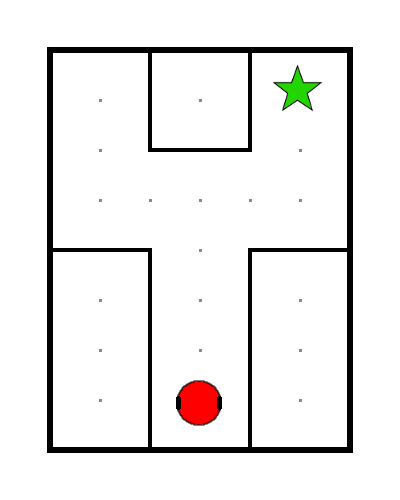
\includegraphics[width=\textwidth]{diagrams/maze_configuration_1}
    \caption{Configuration 1}
    \label{fig:maze_configs/1}
  \end{subfigure}
  ~
  \begin{subfigure}[b]{0.3\textwidth}
    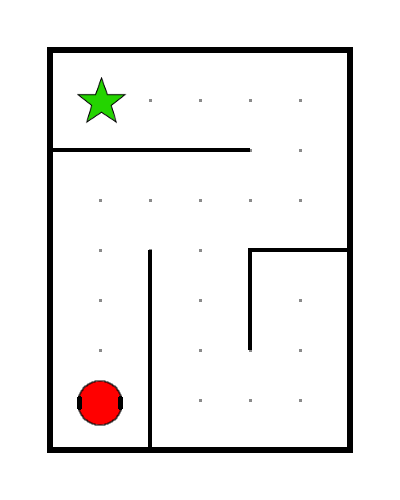
\includegraphics[width=\textwidth]{diagrams/maze_configuration_2}
    \caption{Configuration 2}
    \label{fig:maze_configs/2}
  \end{subfigure}

  \begin{subfigure}[b]{0.3\textwidth}
    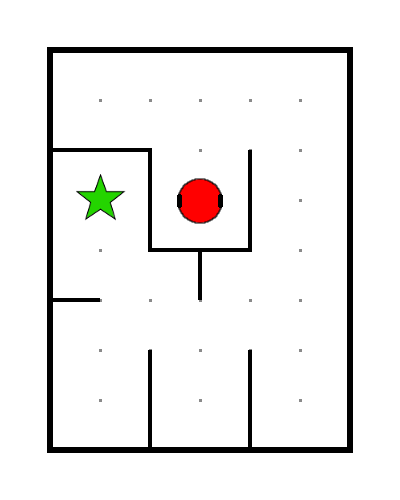
\includegraphics[width=\textwidth]{diagrams/maze_configuration_3}
    \caption{Configuration 3}
    \label{fig:maze_configs/3}
  \end{subfigure}
  ~
  \begin{subfigure}[b]{0.3\textwidth}
    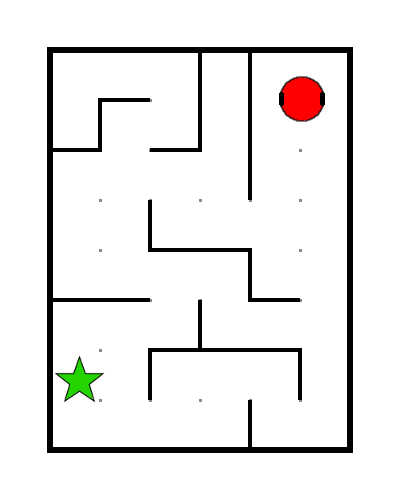
\includegraphics[width=\textwidth]{diagrams/maze_configuration_4}
    \caption{Configuration 4}
    \label{fig:maze_configs/4}
  \end{subfigure}
  \caption{Example Maze Configurations}\label{fig:maze_configs}
\end{figure}

\todo{table goes off the page?}

\begin{table}[!ht]\centering
\caption{Results
\label{results}}
    \begin{tabular}{cccccc}
        \toprule
        \thead{Maze Configuration} & \thead{Number of Agents} & \thead{Run 1[\si{\second}]} & \thead{Run 2[\si{\second}]} & \thead{Run 3[\si{\second}]} & \thead{Avg. Time Taken[\si{\second}]}\\
        \midrule
        1 & 1 & 109.0 & 41.4 & 23.0 & 57.8\\
        1 & 2 & 20.4 & 37.9 & 9.7 & 22.7\\
        2 & 1 & 34.6 & 71.0 & 150.0 & 85.2\\
        2 & 2 & 79.0 & 137.0 & 29.7 & 81.9\\
        3 & 1 & 51.1 & 110.0 & N/A & 80.6\\
        3 & 2 & 60.3 & 82.0 & N/A & 71.2\\
        4 & 1 & 180.4 & 88.0 & N/A & 134.2\\
        4 & 2 & 138.3 & N/A & N/A & 138.3\\
        \bottomrule
    \end{tabular}
\end{table}

The results shown are not indicative of the project had it been completed in its 
entirety, however these results give benchmark scores for the shown maze 
configurations with what is a very basic AI module. A major drawback of the lack of SLAM/AI integration is that the same path can be searched multiple times, which resulted in a few instance with unusually slow results. The results do broadly show, however, 
that multiple agents perform better than a single agent in terms of speed of 
the search. In these cases, this is a simple case of ``many hands make light 
work'' rather than anything intelligent that the robots are doing. 
Nevertheless, the results demonstrate the successful outcomes of the project 
and vindicate the time taken to research the field of co-operative robotics. 
Work detailed in further work (Section~
\ref{furtherwork}) can use the results shown here as benchmark results and 
measure the success of SLAM and AI implementations against these results to 
evaluate progress being made. 

    % !TEX root = ../report.tex

\chapter{Evaulation}\label{eval}
Based on the original objectives of the project (see Section~\ref{introduction/objectives}), the project can be deemed as somewhat of a success. 5 out of 6 of 
the original ``Major'' objectives have been completed, as well as 1 of 2 of 
the ``Optional'' objectives. In addition to this, it is believed that with a 
small number of additional weeks, the two remaining ``Major'' objectives could 
be completed. Given the project as a whole aimed to combine 3 engineering 
disciplines and tackle a number of complex problems simultaneously, a strong 
effort has been made. 
As detailed in various previous sections of the report, a number of small setbacks in 
various aspects of the project caused some of the latter stages of the project to be 
uncompleted. This was especially true as many of the latter elements were sequential, 
and the issues with the EKF resulted in large delays in the SLAM implementation. 

Despite these setbacks, the management of the project was effective and the  tasks were predominantly completed to schedule in the early to middle 
stages of the project. Less management of the project was required in the latter 
stages as objective related tasks became sequential, and those who weren't 
working on those tasks were assigned secondary objectives such as those 
pertaining to the trade show or the report. Git was used effectively, with the 
issues feature and protected merging used to ensure all members of the team were 
working on a task and completion of tasks could be monitored by the project 
manager. 

A series of benchmark results have also been obtained and can be used by future 
iterations of the project to measure success. The 
objectives which have been completed were also iterated upon multiple times to 
complete for each of the robots, and hence the design has 
been improved by using an iterative design process. 

\section{Mechanical}\label{eval/mech} 
Mechanical aspects of the project have been completed to a 
high standard as is demonstrated by the robustness of the robots when in 
motion and the durability and modularity of the maze. This is largely due to the 
decision to complete these tasks first with a higher priority and allow time for the 
designs to be iterated upon throughout the project. The first robot was carefully 
designed to ensure each component mechanically integrated well. This was further 
iterated upon and improved between robots, leading to a final construction which was 
consistent and reliable. Given not all objectives were met at the end of the project 
--- and the electrical and software aspects were to be the focus --- the decision taken in the 
early stages to purchase a pre-built chassis as opposed to create a bespoke chassis 
was justified, due to the time saved. This would have added unnecessary complication 
in the beginning of the project which could have caused future 
tasks to be delayed further. 

The only issue which was encountered with the pre-built chassis was the 
accompanying motors, which were identified as the possible cause of 
issues throughout the electrical and software implementations. When used 
for a reasonable period of time, the motors began to leak grease from 
their plastic casing. This meant that the gearing system was not greased 
and resulted in gears grinding and occasionally slipping. As the 
encoders are on the motor shaft and not the drive shaft, this affected 
the feedback from the encoders. It is thought that this contributed to 
increased differences between robots at the end of the project and 
increased difficulty in tuning the PID controller. This could have been 
mitigated sooner by applying more grease, however this would have meant 
opening the casing of each motor as opposed to just two. If this issue 
had been known from the start, the motors would have been either rotated 
in testing to balance the degradation, or different motors would have 
been used with a bespoke chassis, as finding motors to fit the pre-
existing chassis would not have been a suitable solution. 

Aside from the robots, the other main mechanical component was the modular maze 
testing environment. Although constructed by the mechanical workshop, a great deal of 
effort was put into the design and subsequent iterations to obtain the best outcome 
possible. The modular maze is a reusable ``SLAM playground'' and is a major 
successful outcome of the project. Although not particularly transportable, the maze 
is robust and durable and intended to last --- and be used --- for future projects.

In addition, although not used in the final design, a great deal was learned from 
using CAD to create designs of pegs which were intended for use in the maze. A number 
of iterations of the design were created, which were  improved  both due to the feedback from the mechanical workshop as the specification changed and as the proficiency of using the CAD software increased. It was also worth noting that the CAD designed pegs were not flawed
because of a design flaw, but due to limitations in the printing/construction process and as a result were unusable. 
The mechanical portion of the project can therefore overall be deemed a success as 
the individual components were made to a high standard of design and construction. 

\section{Electrical}\label{eval/elec}
The electrical components of the project were completed to a high standard, 
however some unforeseen complications, caused the completion of these to be delayed.

The pre-built power distribution board chosen had several advantages over a 
custom built solution. Firstly, it was very easily integrated with the Polulu 
chassis. Secondly, it saved the significant amount of time it would have taken 
to build the drive circuit. Lastly, due to manufacturing restrictions on the PCB, 
there was very little remaining space on the system's main PCB, so using a custom 
build system would have required the design of a second. 

The range sensors used proved to be largely successful, with some caveats. 
During the unit testing phase, the sensors performed well, giving consistent 
readings that were accurate to within our required uncertainty. During the SLAM testing, 
they mostly measured accurate results, however, their limitations started to 
become apparent. As the distance increased, the widening cone of detection caused some 
erroneous data to be measured. This is assumed to be the cause of the corners 
appearing to be rounded in the maze in Figure~\todo{reference slam diagram}. 
Another issue with using the ultrasonic sensors is that the RPi used a time 
shared OS, which meant that the readings from timing the pulse from the 
ultrasonic sensor are sometimes inexact. This could be improved with the use of 
a dedicated timing circuit. Finally, as there were several range sensors on each 
robot, taking one measurement sweep took a relatively long time. This is 
especially the case when multiple robots are synchronising their sweeps to avoid 
interference. This would have been mitigated if we had used an infrared sensor. 
This would cost more, but it could be possible to mount the sensor on a servo 
motor, and move it through \ang{180} sweeps as to not require more than one. 
This would also remove the timing issue, as they generally return an analogue 
voltage instead of a pulse time. Initially, this design concept was discounted  due to the additional mechanical complexities of mounting the components and 
cost, however without the time and budget restrictions, this solution would 
likely improve the system's performance. 

While using an IMU to supplement wheel odometry is a common solution, its 
effectiveness in this project has not been proven. The IMU 
returned reasonable results in testing, and the visualisation produced using 
IMU data integrated with ROS shows promise. However, as the EKF is not 
functioning correctly, the sensor-fused results have not been obtained to 
measure their accuracy. 
\todo{Now EKF kind of works can we change this}

Having multiple robots allowed an 
iterative design process to be carried out, significantly improving the outcome 
of the PCB. Connections and vias were altered following the first design to be 
more easily integrable with the mechanical layout.

Time and care was take to ensure the electrical design of the PCB and any other 
connections between parts on the robot --- such as the ribbon cable connection 
between the PCB and the Raspberry Pi --- were robust and correct. This resulted 
in a robot which is both electrically and mechanically sound and replicable 
easily with time and parts. The robots which possess prototype parts, used in 
interim stages of the iterative design process, remain functional and usable. 
This demonstrates the careful selection and design of each of the parts. 

The use of AA batteries throughout the middle stages of the project when the PID 
controller was being tuned, resulted in a great deal of batteries being consumed. 
This was due to the high current spikes which were being caused by motor stalls and 
fewer batteries could have been used if this prolonged process had been foreseen. The 
consistent current draw of the motors throughout this phase of testing should have 
been monitored more closely and action to prevent this taken sooner.   

Overall, the electrical portion of the project was carried out effectively but did 
cause some delays which had a knock on effect later in the project. A number of 
blocking tasks in the middle stages of the project required unforeseen parts to be 
ordered such as ribbon cable and 40-pin IDC connectors which it was thought would 
be found within the department. This was not the case as 40-pin ribbon cable and 
connectors are used predominantly for Raspberry Pis, making them more expensive 
and therefore, not a common order for the department. Hence, these parts had to be ordered in and resulted in the task blocking 
others longer than expected as these were required for system testing. Towards the end of the project, a Raspberry Pi was 
shorted --- the cause is unknown, despite investigations and testing --- and ceased to function, 
meaning time was lost to finding the cause of this issue.    
 
\section{Software}\label{eval/soft}
The software architecture was well designed and thought-out making use of the 
libraries and tools available. By using the ROS library, the architecture was predominantly handled
and did not need to be managed further. Using the ROS library also provided 
access to other tools and libraries such as ``differential-drive'', ``robot-
localization'' and ``g-mapping''. It was thought that these libraries would be ``plug 
and play'' with the modules created as part of the Electrical sections. Despite  
designing and implementing the Electrical modules to integrate with these libraries, 
problems were still encountered with integration. 

The libraries were far more complex than first thought and were also not designed for 
the configuration of sensors used in this project. Additional modules had to be 
created as ``adapters'' with additional parameters between the libraries and the 
originally created modules. Each of the libraries used therefore also had to be fully 
understood, at a source code level, in order to construct the ``adapters'' and alter 
the original modules. This took longer than expected, however did result in more in 
depth knowledge of each of the component parts of the software. As the libraries were 
designed for a variety of other sensors, mainly LIDAR instead of ultrasound, the 
results obtained were not of as high quality as expected and this impacted the time 
taken to tune parameters to achieve the best possible outcome. Although this was 
somewhat achieved for SLAM, this left no time in the project to convert the SLAM map 
to a world state which could then be used by an implemented AI to solve the maze 
intelligently. 

Furthermore, the combination of packages and demanding software made it very difficult to run all the code at once on the Raspberry Pi. The ROS framework together with demanding functions like SLAM and Sensor Fusion proved to be too much for the limited memory and processing power, which made testing fully integrated systems extremely challenging.



    % !TEX root = ../report.tex

\chapter{Further Work}\label{furtherwork}

    % !TEX root = ../report.tex

\chapter{Conclusion}\label{conclusion}

As previously mentioned, tasks that can be parallelised can be solved more 
effectively by using multiple co-operating robots, such as exploration of a large 
area. However, in some environments, such as underground or in areas of high 
interference, communication is severly restricted and the robots would not be able
to co-operate to complete their task. Furthermore, usually systems of co-operating robots 
use a centralised control node to coordinate. Our system was designed so each robot was 
homogenous and operated without this central control unit. This introduced reduncency, 
which is important given the dangerous environments they could be used in, allowing 
the remaining robots to complete the task in the event of the failure of another. 
The robots were also designed to strictly only be able to communicate with other robots 
when they had line-of-sight with each other to simulate potentially restrictive 
environments.  

The mechanical design and implementation of each of the robots can be deemed as 
successful as our key requirements were met. To ensure the system was  
scalable the mechanical design had to be accurately reproduced. This would allow the 
software to be used to be across all the robots without any alterations needed. As a 
result, choosing to use a pre-built chassis was the correct decision. Although given 
the unforeseen issues with regards the reliability of the Pololu kit, the 
requirements to restrict the total cost means there likely is not a better 
alternative. Similarly, the mechanical design of the modular maze environment can 
also be deemed successful. It allowed the system to be tested easily on
different maze configurations, which was essential for the project. Although it took 
longer than expected to produce the maze, it is of a very high quality, is extremely 
customisable and can be reused for any similar projects in the future.

Although issues arose in the process, the end products of the electric deisgn
and implementation were of a high standard. The decision to use the chassis'
accompanying power distrubtion board was justified as it fit both
mechanically and electronically with the other parts, allowing other areas to be 
prioritised. Using ultrasonics was the best method of range detecting even if
they are not perfect due to their wide cone of detection and
cost compared to infrared sensors. The 6-DOF IMU and encoders successfully
provided the neccessary odometry data to track the robot's movements around the
maze. The design of the PCB can also be deemed a success. Although multiple 
iterations of the PCB were designed to improve on the original design, the
thorough planning and design resulted in the first PCB stil being fully functional 
and not needing replaced. 

Ultimately, the decision to use ROS was justified due to it being able to handle
the overall architecture of the system with the publish/subscribe data model
whilst providing accompanying libraries that provide some of the required 
functionality. Although intergrating these libraries was not as simple as 
initially thought, they provided a greater level of functionality than if 
everything was implemented from scratch. The communication module was a great
success with the testing showing it to be extremely thread-safe and allows for
the robots to always being listening for incoming messages. The computer vision
node also works fully within the constraints of the maze. For use in more complex 
environments, a more detailed computer vision would be required.

In summmary, the project delivered the majority of the objectives intitially set
out where each individual components was designed, implemented and tested. Delays
and unforeseen complications resulted in the AI modules not being fully implemented. 
In addition, the complexity of SLAM results in this only being possible at lower 
resolutions, coupled with the uncertainty and timeouts from the ultrasonic sensors, 
the results for this were not as accurate as anticipated. However with greater 
processing power and more time, it is believed this would have performed better.
Despite these issues, the success of each of the earlier components
such as the mechanical and electrical design, the communication software, odometry 
software and computer vision results in the project being overall very successful.

    \pagestyle{plain}
    \bibliographystyle{ieeetr}
    \bibliography{references}

    \appendix{}
    % !TEX root = ../report.tex

\chapter{Some stuff to go after the main report}\label{appendix/a}

The code for this project can be found at:
\begin{center}
https://github.com/rddunphy/CRUES
\end{center}

The directory structure is as follows: 

\begin{itemize}
	\item[] \textbf{docs}: Documentation
		\begin{itemize}
			\item[] \textbf{final}: Latex files of interim report
			\item[] \textbf{interim}: Latex files of interim report
			\item[] \textbf{img}: images used in both reports
		\end{itemize}
	\item[] \textbf{rviz}: Rviz configuration files
	\item[] \textbf{wiring}: Hardware Design Files including PCB files
	\item[] \textbf{crues\_pi}: Source Code
		\begin{itemize}
			\item[] \textbf{config}: Contains each robot's YAML config files
			\item[] \textbf{crues}: Contains helper scripts
			\item[] \textbf{ros\_pkgs}: Contains the directories of the ROS packages
			\item[] \textbf{deploy.sh}: Script to deploy code to RPis
		\end{itemize}
\end{itemize}

\end{document}
